\documentclass[12pt,openany,a4,usenames,dvipsnames]{book}
  \usepackage{polyglossia}
  \usepackage{fontspec}
  \setmainlanguage{english}
  \setotherlanguage{greek}
  \setmainfont{Redaction}
  \usepackage{unicode-math}
  %\setmathfont{Latin Modern Math}
  \setmathfont{TeX Gyre Schola Math}
  \setmonofont[Scale=1.1]{CMU Typewriter Text}
  \newfontfamily\pixelfont{Redaction35-Regular}
  \newfontfamily\fira[Scale=0.90]{Fira Sans}
  \newfontfamily\thumbfont[Scale=0.9]{Redaction35-Bold}
  \newfontfamily\pixeltitle[Scale=3.5]{Redaction35-Bold}
  \newfontfamily\reduxtitle[Scale=3.5]{Redaction-Bold}
  \newfontfamily\cm{CMU Serif}
  \newfontfamily\symbola[Scale=5]{Symbola}
  \usepackage{microtype}
  \usepackage{graphicx}
  \usepackage{dot2texi}
  \usepackage[breaklinks=true]{hyperref}
\hypersetup{
    unicode,
    verbose=false,
    pdfpagelayout=TwoColumnRight,
    bookmarksopen,
    colorlinks,
    citecolor=black,
    filecolor=black,
    linkcolor=black,
    urlcolor=black
}
\usepackage{wrapfig}
\usepackage[nobiblatex]{xurl}
\usepackage{makeidx}
\makeindex
\usepackage[totoc]{idxlayout}
  \usepackage{microtype}
  \usepackage[perpage,symbol*]{footmisc}
  \usepackage{marginnote}
  \usepackage[noclrdblpg]{colophon}
  \usepackage{bookmark}
  \usepackage{amsmath}
  \usepackage{float}
  \usepackage{skeldoc}
  \floatplacement{figure}{H}
  \usepackage{tikz}
  \usepackage{svg}
  \usepackage{calc} % for inkscape pdf tex
  \usepackage{attachfile2}
%\usepackage[showframe,marginparwidth=3cm,twoside=true]{geometry}
\usepackage[marginparwidth=3cm,twoside=true,a4paper]{geometry}
  \usepackage{metalogo}
  \usepackage{csquotes}
  \usepackage[compact,nostruts,medium,noindentafter]{titlesec}
  \newcommand{\chapterbreak}{}
  %\titlespacing*{\chapter}{0pt}{0pt}{0pt}
  \newcommand\makeskelfig{%
    \begin{figure}[H]
  {\centering%
  \skelfig[width=0.4\textwidth]{2\baselineskip}%
  \skelcaption[width=0.2\textwidth,lines=1]{}}
  \end{figure}}
  \usepackage{setspace}
  \definecolor{blackoutline}{RGB}{14,14,14}
  \definecolor{bgcolor}{rgb}{0.95,0.95,0.95}
  \definecolor{red}{rgb}{1,0,0}
  \definecolor{gray}{RGB}{24,24,24}
   \definecolor{thered}    {rgb} {0.65,0.04,0.07}
 \definecolor{thegreen}  {rgb} {0.06,0.44,0.08}
 \definecolor{theblue}   {rgb} {0.02,0.04,0.48}
 \definecolor{sectioning}{gray}{0.44}
 \definecolor{thegrey}   {gray}{0.5}
 \definecolor{theframe}  {gray}{0.75}
 \definecolor{theshade}  {gray}{0.94}
 \definecolor{thepeach}  {RGB}{246,232,220}
 \definecolor{punchbg}{RGB}{250, 230, 180}
 \definecolor{punchframe}{RGB}{240, 220, 170}
\usepackage[cache=false,outputdir=build]{minted}
\setminted[rust]{labelposition=bottomline,bgcolor=thepeach,rulecolor=punchframe,fontsize=\scriptsize,baselinestretch=0.5,frame=leftline,breaklines=true,breakanywhere=true}
\setminted[c]{bgcolor=theshade,fontsize=\scriptsize,baselinestretch=0.5,frame=leftline,breaklines=true,breakanywhere=true}
%\setminted[tex]{breaklines=true,linenos=true,bgcolor=theshade,frame=single,framesep=5pt,rulecolor=theframe}
%\setminted[shell]{breaklines=true,linenos=true,bgcolor=theshade,frame=single,framesep=5pt,rulecolor=theframe}
%\definecolor{bg}{rgb}{0.95,0.95,0.95}
\usepackage{xspace}
\usepackage{xparse}
\usepackage{contour}
\usepackage[normalem]{ulem}
\usepackage{minted}
\usemintedstyle{bw}

\ExplSyntaxOn
\NewDocumentCommand{\TitleOutline}{m}
 {
  \seq_set_split:Nnn \l_tmpa_seq { ~ } { #1 }
  \seq_map_inline:Nn \l_tmpa_seq { \contour{blackoutline}{##1} ~ } \unskip
 }
\ExplSyntaxOff

\renewcommand{\ULdepth}{1.8pt}
\contourlength{0.8pt}

\makeatletter
\renewcommand\@dotsep{200}
\renewcommand{\l@chapter}{\@dottedtocline{0}{0pt}{2.6em}}
\renewcommand{\l@section}{\@dottedtocline{1}{1.5em}{2.6em}}
\renewcommand{\l@subsection}{\@dottedtocline{2}{4.0em}{3.6em}}
\renewcommand{\l@subsubsection}{\@dottedtocline{3}{7.4em}{4.5em}}
\makeatother

\newcommand\bitmap{{\pixelfont{}bitmap}}
\newcommand\bitmaps{{\pixelfont{}bitmaps}}
\newcommand\pixel{{\pixelfont{}pixel}}
\newcommand\pixels{{\pixelfont{}pixels}}
\newcommand\Rust{{\fira{}\textbf{Rust}}}

\newcommand\colorunderline[1]{\bgroup\markoverwith{\textcolor{#1}{\rule[-0.5ex]{2pt}{0.8pt}}}\ULon}
\newcommand{\myuline}[2]{%
  \colorunderline{#1}{\phantom{#2}}%
  \llap{\contour{white}{#2}}%
}
\DeclareRobustCommand{\myurl}[2]{%
  \href{#1}{\myuline{blue}{#2}}%
}

\newcommand{\attachsource}[1]{%
\marginnote{\scriptsize{}%
\texttt{\tiny{}#1}:\\
\attachfile[icon=Paperclip]{#1}\hfill\\
This code file is a PDF attachment}%
}%
\DeclareRobustCommand{\sourceinlib}{%
\marginnote{\scriptsize{}%
This code is included in the distributed library file in the \emph{\nameref{ch:intro-library}} chapter.}%
}%
\newcommand\titletext{A {\pixeltitle{}Bitmapper}'s Companion}
\newcommand\covertitletext{\TitleOutline{A {\pixeltitle{}Bitmapper}'s Companion}}
\title{\titletext{}}
\newcommand\subtitle{an introduction to basic \bitmap{} mathematics and algorithms with code samples in \Rust{}}
\newcommand\coversubtitle{\TitleOutline{an introduction to basic \bitmap{} mathematics and algorithms with code samples in \Rust{}}}
\newcommand\biblatex{\texttt{biblatex}\xspace}%
\hypersetup{
  pdftitle={\titletext{}},
  pdfauthor={epilys},
  pdfsubject={programming},
}
\usepackage{wallpaper}

\newsavebox{\mintedbox}

\usepackage[thumblink=line,height=50pt,minheight={50pt},width=50pt,distance={2mm},topthumbmargin={5cm},bottomthumbmargin={2pt},eventxtindent={0pt},oddtxtexdent={2pt},evenmarkindent={0pt},oddmarkexdent={0pt},evenprintvoffset={0pt},nophantomsection=false,ignorehoffset=true,ignorevoffset=true,final=true,hidethumbs=false,verbose=true]{thumbs}
 \definecolor{ThumbBg}  {rgb} {0.2,0.2,0.2}
 \definecolor{DarkBg}  {rgb} {0.17,0.17,0.17}
 \definecolor{DarkFg}  {rgb} {0.90,0.90,0.90}
 \definecolor{LightBg} {rgb}{1.0,1.0,1.0}
\newcommand{\setbackgroundcolour}{\pagecolor{DarkBg}}
\newcommand{\settextcolour}{\color[rgb]{0.90,0.90,0.90}}
\newcommand{\invertbackgroundtext}{\setbackgroundcolour\settextcolour}
\newcommand{\revertbackgroundcolour}{\pagecolor{LightBg}}
\newcommand{\reverttextcolour}{\color[rgb]{0.19,0.19,0.19}}
\newcommand{\revertbackgroundtext}{\revertbackgroundcolour\reverttextcolour}

\newcommand\myaddthumb[2]{%
  %\addtitlethumb{#1}{\fcolorbox{red}{black}{\parbox[t][45pt]{45pt}{\noindent%
  \addtitlethumb{\hspace{5pt}#1}{%
    \parbox[t][43pt]{43pt}{\centering
    \vfill\noindent%
{\linespread{.7}\thumbfont{}#2\par\vfill}%
}%
}{white}{ThumbBg}{pagesLTS.0}%
}%

\pagenumbering{arabic}

  \usepackage[textsize=tiny]{todonotes}



\DeclareRobustCommand{\Caption}[1]{\par%
  \vspace{1em}
  {\noindent{}#1}}

\usepackage{scalerel}

\DeclareRobustCommand\archat[1]{%
\begin{array}{c}
\stretchto{
  \scaleto{
    \scalerel*[\widthof{#1}]{\frown}
    {\rule[-\textheight/2]{1ex}{\textheight}} %WIDTH-LIMITED BIG WEDGE
  }{1.25\textheight} % THIS STRETCHES THE WEDGE A LITTLE EXTRA WIDE
}{0.5ex}\\           % THIS SQUEEZES THE WEDGE TO 0.5ex HEIGHT
#1\\                   % THIS STACKS THE WEDGE ATOP THE ARGUMENT
\rule{0ex}{.01ex}
\end{array}
}

\DeclareRobustCommand\TheEnd{%
\par%
\thispagestyle{empty}%
{\vfill{}\noindent{}\centering{}\symbola{}⸎\par}%
}

\begin{document}
\pagestyle{plain}
  \assignpagestyle{\chapter}{plain}
\newgeometry{left=1cm,top=0.1cm,right=1cm,bottom=0.1cm}
\pdfbookmark{Title page}{title-page}%cover
\ThisLRCornerWallPaper{0.55}{figures/Holbein_Skull2_inverted.png}
\setstretch{1.1}
\invertbackgroundtext
\addtolength{\parskip}{5pt}%
\newlength\drop
\thispagestyle{empty}
\begingroup% Harry Carter
\setlength{\drop}{0.1\textheight}
\vspace*{\drop}
\begin{flushleft}
  \textcolor{thegrey}{\rule{\textwidth}{1.6pt}}%
  \vspace{-0.9\baselineskip}
  \textcolor{sectioning}{\rule{\textwidth}{0.4pt}}\\[0.8\baselineskip]
  {\centering
  \contourlength{0.02em}
  \scalebox{2.0}{\parbox{0.5\textwidth}{\centering{\reduxtitle{}\covertitletext{}}}}\\
  \vspace{.8\baselineskip}
  \par
  \vspace{-0.4\baselineskip}
  }\textcolor{thegrey}{\rule{\textwidth}{1.6pt}}%
  \vspace{-0.9\baselineskip}
  \textcolor{sectioning}{\rule{\textwidth}{0.4pt}}\\[0.2\baselineskip]
  {\Large{}\TitleOutline{epilys}}\hfill{\small{}\TitleOutline{2021}}
  \vfill%
  \scalebox{1.5}{\parbox{0.28\textwidth}{\noindent%
  {\LARGE\raggedleft\coversubtitle{}\par}
  }}
  \vfill%
\end{flushleft}%
\endgroup
\clearpage{}
\restoregeometry
\revertbackgroundtext
\clearpage{}
\thispagestyle{empty}
.
\clearpage{}
\thispagestyle{empty}
\thumbsoverview{map}
\clearpage{}
\thispagestyle{empty}
\marginnote{
\includegraphics{figures/xface.png}}[-1.3\baselineskip]\noindent{}Manos Pitsidianakis (epilys)\\
\myurl{https://nessuent.xyz}{https://\-nessuent.xyz}\\
\myurl{https://github.com/epilys}{https://github.com/epilys}\\
\myurl{epilys@nessuent.xyz}{epilys@nessuent.xyz}\\

\noindent{}All non-screenshot figures were generated by hand in Inkscape unless otherwise stated.

\noindent{}The skull in the cover is a transformed \bitmap{} of the skull in the 1533 oil painting by Hans Holbein the Younger, \myurl{https://en.wikipedia.org/wiki/The_Ambassadors_(Holbein)}{\emph{The Ambassadors}}, which features a floating distorted skull rendered in anamorphic perspective.

\noindent{}\emph{A Bitmapper’s Companion}, 2021\\
\noindent{}\textbf{Special Topics} $\blacktriangleright{}$ \textbf{Computer Graphics} $\blacktriangleright{}$ \textbf{Programming}\\
\noindent{}006.6'6--dc20
\vfill{}
\noindent{}Copyright © 2021 by Emmanouil Pitsidianakis

\noindent{}This work is licensed under the Creative Commons Attribution-NonCommercial-ShareAlike 3.0 Unported License. To view a copy of this license, visit\\\myurl{http://creativecommons.org/licenses/by-nc-sa/3.0/}{http\-:\-//\-creativecommons\-.\-org\-/\-licenses\-/\-by-nc-sa/3.0/} or send a letter to Creative Commons, PO Box 1866, Mountain View, CA 94042, USA.

\noindent{}The source code for this work is available under the GNU GENERAL PUBLIC LICENSE version 3 or later. You can view it, study it, modify it for your purposes as long as you respect the license if you choose to distribute your modifications.

\noindent{}The source code is available here

\noindent{}\myurl{https://github.com/epilys/bitmappers-companion}{https://github.com/epilys/bitmappers-companion}

\clearpage{}
\myaddthumb{Table Of Contents}{toc}
\pdfbookmark{\contentsname}{toc}
\ThisLRCornerWallPaper{0.6}{figures/The-Ambassadors.png}
\tableofcontents
\ThisLRCornerWallPaper{0.4}{figures/Holbein_Skull.png}
\clearpage{}
\myaddthumb{Introduction}{intro}
\part{Introduction}
\chapter{Data representation}\label{ch:intro-library}
The data structures we're going to use is \emph{Point} and \emph{Image}. \emph{Image} represents a \bitmap{}, although we will use full RGB colors for our points therefore the size of a \pixel{} in memory will be \texttt{u8} instead of 1 bit.

We will work on the cartesian grid representing the framebuffer that will show us the \pixels{}. The \emph{origin} of this grid (i.e.\ the center) is at $(0,0)$.%
\begin{figure}%
\centering
\input{figures/cartesian_grid.pdf_tex}
\end{figure}%
%
We will represent points as pairs of signed integers. When actually drawing them though, negative values and values outside the window's geometry will be ignored (clipped).
%
\attachsource{src/lib.rs}
%
\begin{minted}{rust}
pub type Point = (i64, i64);

pub const fn from_u8_rgb(r: u8, g: u8, b: u8) -> u32 {
    let (r, g, b) = (r as u32, g as u32, b as u32);
    (r << 16) | (g << 8) | b
}
pub const AZURE_BLUE: u32 = from_u8_rgb(0, 127, 255);
pub const RED: u32 = from_u8_rgb(157, 37, 10);
pub const WHITE: u32 = from_u8_rgb(255, 255, 255);
pub const BLACK: u32 = 0;

pub struct Image {
    pub bytes: Vec<u32>,
    pub width: usize,
    pub height: usize,
    pub x_offset: usize,
    pub y_offset: usize,
}

impl Image {
    pub fn new(width: usize, height: usize, x_offset: usize, y_offset: usize) -> Self;
    pub fn magick_open(path: &str, x_offset: usize, y_offset: usize) -> Result<Self, Box<dyn Error>>;
    pub fn from_xbm(path: &str, x_offset: usize, y_offset: usize) -> Result<Self, Box<dyn Error>>;
    pub fn draw(&self, buffer: &mut Vec<u32>, fg: u32, bg: Option<u32>, window_width: usize);
    pub fn draw_outline(&mut self);
    pub fn clear(&mut self);
    pub fn plot(&mut self, x: i64, y: i64);
    pub fn get(&mut self, x: i64, y: i64) -> u32;
    pub fn plot_ellipse(
        &mut self,
        (xm, ym): (i64, i64),
        (a, b): (i64, i64),
        quadrants: [bool; 4],
        _wd: f64,
    );
    pub fn plot_line_width(&mut self, point_a: Point, point_b: Point, wd: f64);
    pub fn flood_fill(&mut self, mut x: i64, y: i64);
}
\end{minted}

An RGB color with coordinates $(r, g, b)$ where $r, g, b: \textrm{\texttt{u8} values}$ is represented as a \texttt{u32} number with the red component shifted 16 bits to to the left, the green component 8 bits, and the final 8 bits are the blue component. It's essentially laying the $r, g, b$ values sequentially and forming a 32 bit value out of three 8 bit values.

Our \texttt{Image::plot(x, y)} function sets the $(x, y)$ pixel to black. To do that we set the element \texttt{y * width + x} of the \texttt{Image's} buffer to the black color as RGB.

\chapter{Displaying {\pixels{}} to your screen}
A way to display an \emph{Image} is to use the \texttt{minifb} crate which allows you to create a window and draw \pixels{} directly on it. Here's how you could set it up:
%
\attachsource{src/bin/introduction.rs}
%
%
\begin{minted}{rust}
use bitmappers_companion::*;
use minifb::{Key, Window, WindowOptions};

const WINDOW_WIDTH: usize = 400;
const WINDOW_HEIGHT: usize = 400;

fn main() {
    let mut buffer: Vec<u32> = vec![WHITE; WINDOW_WIDTH * WINDOW_HEIGHT];
    let mut window = Window::new(
        "Test - ESC to exit",
        WINDOW_WIDTH,
        WINDOW_HEIGHT,
        WindowOptions {
            title: true,
            //borderless: true,
            //resize: false,
            //transparency: true,
            ..WindowOptions::default()
        },
    )
    .unwrap();

    // Limit to max ~60 fps update rate
    window.limit_update_rate(Some(std::time::Duration::from_micros(16600)));

    let mut image = Image::new(50, 50, 150, 150);
    image.draw_outline();
    image.draw(&mut buffer, BLACK, None, WINDOW_WIDTH);

    while window.is_open()
         && !window.is_key_down(Key::Escape)
         && !window.is_key_down(Key::Q) {
        window
            .update_with_buffer(&buffer, WINDOW_WIDTH, WINDOW_HEIGHT)
            .unwrap();
        let millis = std::time::Duration::from_millis(100);
        std::thread::sleep(millis);
    }
}
\end{minted}

Running this will show you something like this:
% FIXME reduce window size and resulting screenshot size

\begin{figure}[H]
\centering
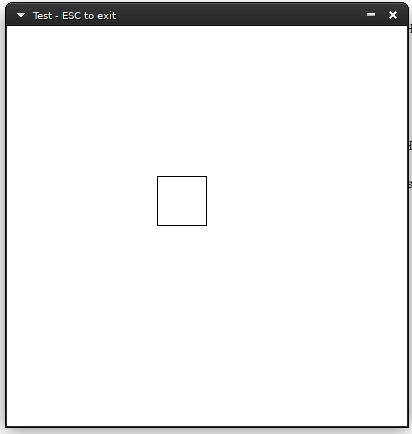
\includegraphics{figures/introduction.png}
\end{figure}

By drawing each individual pixel with the \texttt{Image::plot} and \texttt{Image::plot\_color} functions, we can draw any possible RGB picture of the buffer size. In this book's chapters, we will usually calculate pixels by using discrete calculations of each pixels as integers, or by using rational values (with 64 bit floating point representation) and then calculating their integer values with the \texttt{floor} function. This can also be done by casting an \texttt{f64} type to \texttt{i64} with \texttt{as}: 

\begin{minted}{rust}
  let val: f64 = 5.5;
  let val: i64 = val as i64;
  assert_eq!(5i64, val);
\end{minted}

\chapter{Bits to byte \pixels{}}\label{ch:bitstobytes}
If we worked with 1 bit images (black and white) it could be a more space-efficient representation to store the pixels as bits: 8 pixels in 1 byte. For this book we accept that our images can have RGB colors. The \texttt{xbm} format stores pixels like that, and we might wish to convert them to our representation.

Let's define a way to convert bit information to a byte vector:

\begin{minted}{rust}
pub fn bits_to_bytes(bits: &[u8], width: usize) -> Vec<u32> {
    let mut ret = Vec::with_capacity(bits.len() * 8);
    let mut current_row_count = 0;
    for byte in bits {
        for n in 0..8 {
            if byte.rotate_right(n) & 0x01 > 0 {
                ret.push(BLACK);
            } else {
                ret.push(WHITE);
            }
            current_row_count += 1;
            if current_row_count == width {
                current_row_count = 0;
                break;
            }
        }
    }
    ret
}
\end{minted}

\chapter{Loading graphics files in \Rust{}}
The book's library includes a method to load \texttt{xbm} files on runtime (see \emph{\nameref{ch:xbmtors}} for including them in your binary at compile time). If your system has \texttt{ImageMagick} installed and the commands \texttt{identify} and \texttt{magick} are in your \texttt{PATH} environment variable, you can use the \texttt{Image::magick\_open} method:

\begin{minted}{rust}
  impl Image {
    ...
    pub fn magick_open(path: &str, x_offset: usize, y_offset: usize) -> Result<Self, Box<dyn Error>>;
    ...
  }
\end{minted}

It simply converts the image file you pass to it to raw bytes using the invocation \texttt{magick convert \emph{path} RGB:-} which prints raw \texttt{RGB} content to \texttt{stdout}.

If you have another way to load pictures such as your own code or a picture format library crate, all you have to do is convert the pixel information to an \texttt{Image} whose definition we repeat here:

\begin{minted}{rust}
pub struct Image {
    pub bytes: Vec<u32>,
    pub width: usize,
    pub height: usize,
    pub x_offset: usize,
    pub y_offset: usize,
}
\end{minted}
\chapter{Including \texttt{xbm} files in \Rust{}}\label{ch:xbmtors}

\emph{The end of this chapter includes a short \Rust{} program to automatically convert \texttt{xbm} files to equivalent \Rust{} code.}

\texttt{xbm} files are C source code files that contain the \pixel{} information for an image as macro definitions for the dimensions and a static \texttt{char} array for the \pixels{}, with each bit column representing a pixel. If the width dimension doesn't have 8 as a factor, the remaining bit columns are left blank/ignored.

They used to be a popular way to share user avatars in the old internet and are also good material for us to work with, since they are small and numerous. The following is such an image:

\begin{figure}[H]
\centering

\includegraphics{figures/news.png}
\end{figure}
%FIXME
Then, we can convert the \texttt{xbm} file from C to \Rust{} with the following transformations:

\begin{minted}{c}
#define news_width 48
#define news_height 48
static char news_bits[] = {
\end{minted}

to


\begin{minted}{rust}
const NEWS_WIDTH: usize = 48;
const NEWS_HEIGHT: usize = 48;
const NEWS_BITS: &[u8] = &[
\end{minted}

And replace the closing \texttt{\}} with \texttt{]}.

We can then include the new file in our source code:


\begin{minted}{rust}
include!("news.xbm.rs");
\end{minted}

load the image:

\begin{minted}{rust}
let mut image = Image::new(NEWS_WIDTH, NEWS_HEIGHT, 25, 25);
image.bytes = bits_to_bytes(NEWS_BITS, NEWS_WIDTH);
\end{minted}

and finally run it:

\begin{figure}[H]
\centering

\includegraphics{figures/intro-2.png}
\end{figure}

The following short program uses the \texttt{regex} crate to match on these simple rules and print the equivalent code in \texttt{stdout}. You can use it like so:

\begin{minted}{shell}
cargo run --bin xbmtors -- file.xbm > file.xbm.rs
\end{minted}
\attachsource{src/bin/xbmtors.rs}

\begin{minted}{rust}
use regex;
use regex::Regex;
use std::fs::File;
use std::io::prelude::*;

fn main() {
    let args = std::env::args().skip(1).collect::<Vec<String>>();
    if args.len() != 1 {
        println!("one argument expected, the xbm file path to convert.");
        return;
    }
    let mut file = match File::open(&args[0]) {
        Err(err) => panic!("couldn't open {}: {}", args[0], err),
        Ok(file) => file,
    };

    let mut s = String::new();
    if let Err(err) = file.read_to_string(&mut s) {
        panic!("couldn't read {}: {}", args[0], err);
    }

    let re = Regex::new(
        r"(?imx)
  ^\s*\x23\s*define\s+(?P<i>.+?)_width\s+(?P<w>\d\d*)$
  \s*
  ^\s*\x23\s*define\s+.+?_height\s+(?P<h>\d\d*)$
  \s*
  ^\s*static(\s+unsigned){0,1}\s+char\s+.+?_bits..\s*=\s*\{(?P<b>[^}]+)\};
",
    )
    .unwrap();

    let caps = re
        .captures(&s)
        .expect("Could not convert file, regex doesn't match :(");
    let ident = caps.name("i").unwrap().as_str().to_uppercase();
    let out = re.replace_all(&s, format!("const {i}_WIDTH: usize = $w;\nconst {i}_HEIGHT: usize = $h;\nconst {i}_BITS: &[u8] = &[$b];", i = &ident));
    println!("{}", out.trim());
}
\end{minted}
\clearpage{}
\myaddthumb{Points And Lines}{lines}
\part{Points And Lines}
\chapter{Distance between two points}\index{distance!between two points}

\begin{figure}[H]
\centering
\input{figures/fig1.pdf_tex}
\end{figure}

Given two points, $K$ and $L$, an elementary application of Pythagoras' Theorem gives the distance between them as

\begin{equation}
  r = \sqrt{(x_{L} - x_{K})^{2} +(y_{L} - y_{K})^{2}}
\end{equation}
which is simply coded:
\begin{minted}{rust}
pub fn distance_between_two_points(p_k: Point, p_l: Point) -> f64 {
    let (x_k, y_k) = p_k;
    let (x_l, y_l) = p_l;
    let xlk = x_l - x_k;
    let ylk = y_l - y_k;
    f64::sqrt((xlk*xlk + ylk*ylk) as f64)
}
\end{minted}
\chapter{Moving a point to a distance at an angle}\index{distance!moving a point}

Moving a point $P=(x,y)$ at distance $d$ at an angle of $r$ radians is solved with simple trigonometry:

$$P'=(x+d\times{}\cos{}r, y+d\times{}\sin{}r)$$

Why? The problem is equivalent to calculating the point of a circle with $P$ as the center, $d$ the radius at angle $r$ and as we will later\footnote{\emph{\nameref{ch:equations-circles}} page \pageref{ch:equations-circles}} see this is how the points of a circle are calculated.

\begin{minted}{rust}
pub fn move_point(p: Point, d: f64, r: f64) -> Point {
  let (x, y) = p;
  (x + (d * f64::cos(r)).round() as i64, y + (d * f64::sin(r)).round() as i64)
}
\end{minted}

\chapter{Equations of a line}\label{ch:equations-lines}\index{line!equations}
There are several ways to describe a line mathematically. We'll list the convenient ones for drawing \pixels{}.

The equation that describes every possible line on a two dimensional grid is the \emph{implicit} form $ax+by=c, (a,b) \neq{} (0,0)$. We can generate equivalent equations by adding the equation to itself, i.e.\ $ax+by=c \equiv 2ax+2by=2c \equiv a'x+b'y=c', a'=2a, b'=2b, c'=2c$ as many times as we want. To "minimize" the constants $a,b,c$ we want to satisfy the relationship $a^{2}+b^{2}=1$, and thus can convert the equivalent equations into one representative equation by multiplying the two sides with $\frac{1}{\sqrt{a^2+b^2}}$; this is called the normalized equation. % TODO: why? add footnote: in the normalized form, a is the cosine of the angle the normal vector makes with the x axis, and b the cosine of the angle with the y axis. and c = - (dist of line to the origin)

The \emph{slope intercept form} describes any line that intercepts the $y$ axis at $b \in{} \mathbb{R}$ with a specific slope $a$:

$$y=ax+b$$

The \emph{parametric} form\ldots{} % TODO

%% TODO: add conversion between forms

\section{Line through a point $P=(x_p,y_p)$ and a slope $m$}\index{line!through point and slope}

$$y-y_p=m(x-x_p)$$

\section{Line through two points}\label{sec:linethroughtwopoints}\index{line!through two points}
\begin{figure}[H]
\centering
\input{figures/line_through_points.pdf_tex}
\end{figure}
It seems sufficient, given the coordinates of two points $M, N$, to calculate $a, b$ and $c$ to form a line equation:

$$ax+by+c=0$$

If the two points are not the same, they necessarily form such a line. To get there, we start from expressing the line as parametric over $t$: at $t=0$ it's at point $M$ and at $t=1$ it's at point $N$:

$$c = c_M + (c_N - c_M)t, t\in R, c \in \{x, y\}$$
$$c = c_M, t\in R, c \in \{x, y\}$$

Substituting $t$ in one of the equations we get:

$$(y_M - y_N)x + (x_N-x_M)y+(x_{M}y_{N}-x_{N}y_{M})=0$$

Which is what we were after. We should finish by normalising what we found with $\frac{1}{\sqrt{a^2+b^2}}$, but our coordinates are integers and have no decimal or floating point accuracy.

\begin{minted}{rust}
fn find_line(point_a: Point, point_b: Point) -> (i64, i64, i64) {
    let (xa, ya) = point_a;
    let (xb, yb) = point_b;
    let a = yb - ya;
    let b = xa - xb;
    let c = xb * ya - xa * yb;

    (a, b, c)
}
\end{minted}
%
%
%
\chapter{Drawing a line}\index{line!drawing}
\begin{minted}{rust}
fn plot_line(image: &mut Image, (a, b, c): (i64, i64, i64)) {
    let x = if a != 0 { -1 * (c) / a } else { 0 };
    let mut prev_point = (x, 0);
    for y in 0..(WINDOW_HEIGHT as i64) {
        // ax+by+c =0 =>
        // x=(-c-by)/a
        let x = if a != 0 { -1 * (c + b * y) / a } else { 0 };
        let new_point = (x, y);
        image.plot_line_width(prev_point, new_point, 1.0);
        prev_point = new_point;
    }
}
\end{minted}
%
%
%
\chapter{Distance from a point to a line}\index{distance!point from a line}
\begin{figure}[H]
\centering
\input{figures/point_line_distance.pdf_tex}
\end{figure}

\section{Using the implicit equation form}
Let's find the distance from a given point $P$ and a given line $L$. Let $d$ be the distance between them. Bring $L$ to the implicit form $ax+by=c$.

$$d= \frac{|ax_p+by_p+c|}{\sqrt{a^2+b^2}}$$

\section{Using an $L$ defined by two points $P_1, P_2$}
With $P=(x_0, y_0)$, $P_1 = (x_1, y_1)$ and $P_2 = (x_2, y_2)$.

$$d=\frac{|(x_2-x_1)(y_1-y_0)-(x_1-x_0)(y_2-y_1)|}{\sqrt{((x_2-x_1)^2+(y_2-y_1)^2}}$$
\section{Using an $L$ defined by a point $P_l$ and angle $\hat{θ}$}

$$d=\left|\cos{}(\hat{θ})(P_{ly}-y_p)-\sin{}(\hat{θ})(P_{lx} - P_x)\right|$$

\section*{The code}
This function uses the implicit form.
\sourceinlib%
\begin{minted}{rust}
type Line = (i64, i64, i64);
pub fn distance_line_to_point((x, y): Point, (a, b, c): Line) -> f64 {
    let d = f64::sqrt((a * a + b * b) as f64);
    if d == 0.0 {
        0.
    } else {
        (a * x + b * y + c) as f64 / d
    }
}
\end{minted}

\chapter{Perpendicular lines}\label{ch:perpendicular}\index{perpendicular}\index{line!perpendicular}
\section{Find perpendicular to line that passes through given point}
Now, we wish to find the equation of the line that passes through $P$ and is perpendicular to $L$. Let's call it $L_{⊥}$. $L$ in implicit form is $ax+by+c=0$. The perpendicular will be:

$$L_{⊥}: bx-ay+(aP_y-bP_x)=0$$

\subsection*{The code}
\sourceinlib%
\begin{minted}{rust}
type Line = (i64, i64, i64);
fn perpendicular((a, b, c): Line, p: Point) -> Line {
    (b, -1 * a, a * p.1 - b * p.0)
}
\end{minted}

\section{Find point in line that belongs to the perpendicular of given point}
\subsection*{The code}
\sourceinlib%
\begin{minted}{rust}
fn point_perpendicular((a, b, c): Line, p: Point) -> Point {
    let d = (a * a + b * b) as f64;
    if d == 0. {
        return (0, 0);
    }
    let cp = a * p.1 - b * p.0;
    (
        ((-a * c - b * cp) as f64 / d) as i64,
        ((a * cp - b * c) as f64 / d) as i64,
    )
}
\end{minted}

% From graphic gems vol 2 pdf page 40
\chapter{Angle between two lines}\index{angle!between two lines}
\begin{figure}[H]
\centering
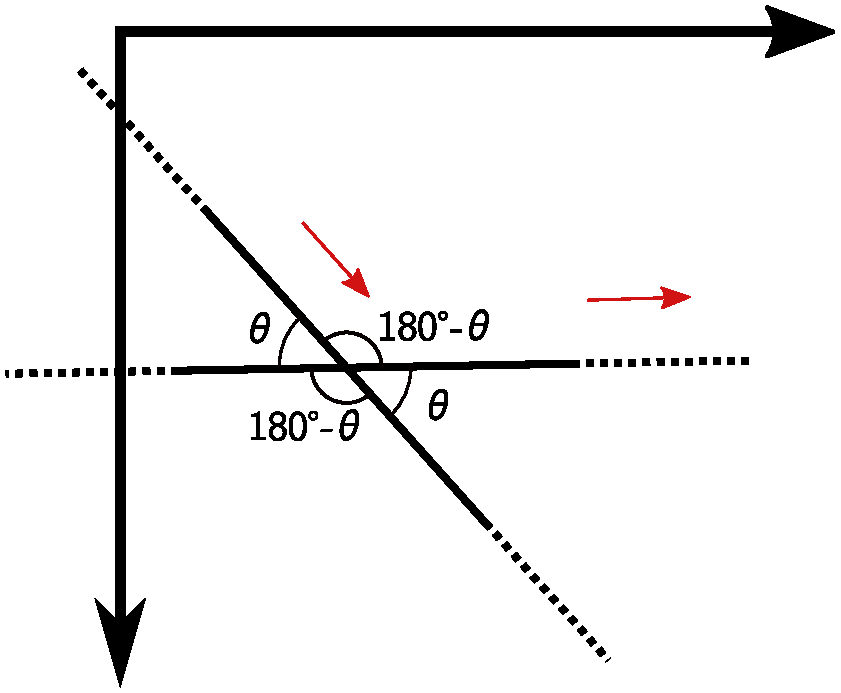
\includegraphics[width=0.6\textwidth,keepaspectratio]{figures/line_angles.pdf}
\end{figure}
By angle we mean the angle formed by the two directions of the lines; and direction vectors start from the origin (in the figure, they are the \textcolor{red}{red arrows}). So if we want any of the other three angles, we already know them from basic geometry as shown in the figure above.

If you prefer using the implicit equation, bring the two lines $L_1$ and $L_2$ to that form ($a_1x+b_1y+c=0$ and $a_2x+b_2y+c_2=0$) and you can directly find $\hat{θ}$ with the formula:
$$\hat{θ} = \arccos{}\frac{a_{1}a_{2}+b_{1}b_{2}}{\sqrt{\left(a_1^2 + b_1^2\right)\left(a_2^2+b_2^{2}\right)}}$$
For the following parametric equations of $L_1$, $L_2$:

$$ L_{1} = \left(\{x=x_1 +f_1t\}, \{y=y_1+g_1t\}\right)$$
$$ L_{2} = \left(\{x=x_2 +f_2s\}, \{y=y_2+g_2s\}\right)$$

the formula is:

$$\hat{θ} = \arccos\frac{f_{1}f_{2}+g_{1}g_{2}}{\sqrt{\left(f_1^2 + g_1^2\right)\left(f_2^2+g_2^2\right)}}$$

\noindent{}The code:

\attachsource{src/bin/anglebetweenlines.rs}
\begin{minted}{rust}
fn find_angle((a1, b1, c1): (i64, i64, i64), (a2, b2, c2): (i64, i64, i64)) -> f64 {
    let nom = (a1 * a2 + b1 * b2) as f64;
    let denom = ((a1 * a1 + b1 * b1) * (a2 * a2 + b2 * b2)) as f64;

    f64::acos(nom / f64::sqrt(denom))
}
\end{minted}
\begin{figure}[H]
  \centering
  \begin{minipage}{0.49\textwidth}
    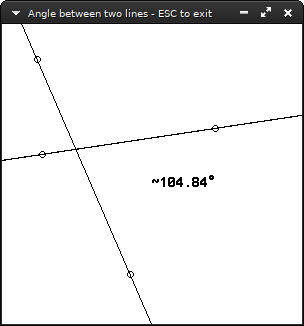
\includegraphics[width=\textwidth,keepaspectratio]{figures/anglelines1.png}
  \end{minipage}
  \hspace{.1em}
  \begin{minipage}{0.49\textwidth}
    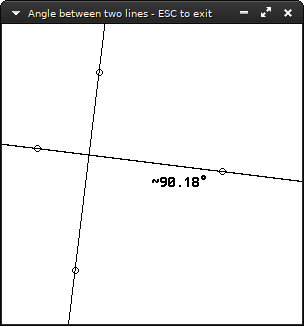
\includegraphics[width=\textwidth,keepaspectratio]{figures/anglelines2.png}
  \end{minipage}
  \Caption{The \texttt{src/bin/anglebetweenlines.rs} example has two interactive lines and computes their angle with 64bit floating point accuracy.}
\end{figure}
%
%
%
%
\chapter{Intersection of two lines}\label{ch:intersection-lines}\index{line!intersection}
\begin{figure}[H]
\centering
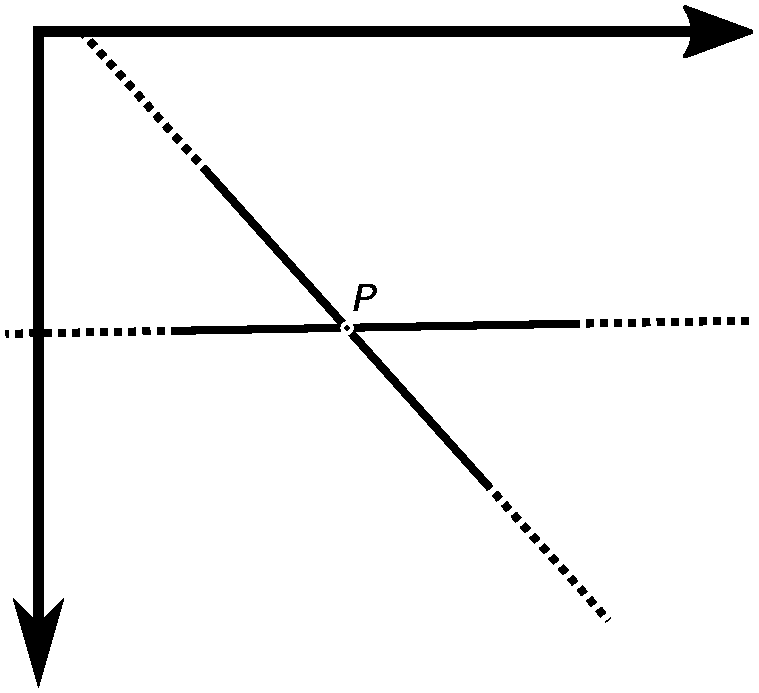
\includegraphics[width=0.6\textwidth,keepaspectratio]{figures/intersection_lines.pdf}
\end{figure}
If the lines $L_1$, $L_2$ are in implicit form ($a_1x+b_1y+c=0$ and $a_2x+b_2y+c_2=0$), the result comes after checking if the lines are parallel (in which case there's no single point of intersection):

$$a_1b_2-a_2b_1 \neq{} 0$$

If they are not parallel, $P$ is:

$$P = \left(\frac{b_1c_2-b_2c_1}{a_1b_2-a_2b_1}, \frac{a_2c_1-a_1c_2}{a_1b_2-a_2b_1}\right)$$

\noindent{}The code:

\attachsource{src/bin/lineintersection.rs}
\begin{minted}{rust}
fn find_intersection((a1, b1, c1): (i64, i64, i64), (a2, b2, c2): (i64, i64, i64)) -> Option<Point> {
    let denom = a1 * b2 - a2 * b1;

    if denom == 0 {
        return None;
    }

    Some(((b1 * c2 - b2 * c1) / denom, (a2 * c1 - a1 * c2) / denom))
}
\end{minted}
\begin{figure}[H]
  \centering
  \begin{minipage}{0.49\textwidth}
    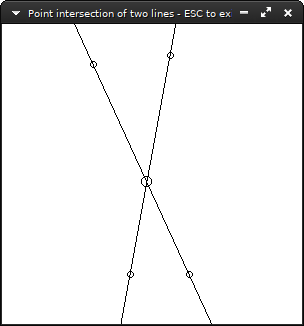
\includegraphics[width=\textwidth,keepaspectratio]{figures/lineintersection1.png}
  \end{minipage}
  \hspace{.1em}
  \begin{minipage}{0.49\textwidth}
    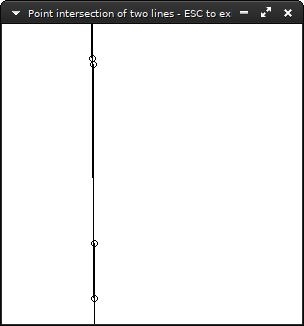
\includegraphics[width=\textwidth,keepaspectratio]{figures/lineintersection2.png}
  \end{minipage}
  \Caption{The \texttt{src/bin/lineintersection.rs} example has two interactive lines and computes their point of intersection.}
\end{figure}
%
%
%
%
\chapter{Line equidistant from two points}\index{line!equidistant}\index{equidistant line}
\begin{figure}[H]
\centering
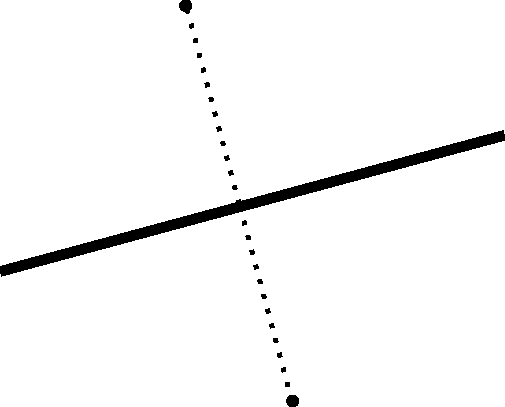
\includegraphics[height=8\baselineskip,keepaspectratio]{figures/equidistant.pdf}
\end{figure}
Let's name this line $L$. From previous chapter\footnote{See \emph{\nameref{sec:linethroughtwopoints}}, page \pageref{sec:linethroughtwopoints}} we know how to get the line $L$ that's created by the two points $M$ and $N$:
%
$$L: (y_M - y_N)x + (x_N-x_M)y+(x_{M}y_{N}-x_{N}y_{M})=0$$%
%
We need the perpendicular line over the midpoint of $L$.\footnote{See \emph{\nameref{ch:perpendicular}}, page \pageref{ch:perpendicular}} The midpoint also satisfies $L$'s equation. The midpoint's coordinates are intuitively:\index{midpoint}

$$P_{mid} = \left(\frac{x_M + x_N}{2}, \frac{y_M + y_N}{2}\right)$$

The perpendicular's $L_{⊥}$ equation is

$$L_{EQ} = L_{⊥}: yx-ay+\left(aP_{mid_y}-bP_{mid_x}\right)=0$$

\noindent{}The code:

\attachsource{src/bin/equidistant.rs}
\begin{minted}{rust}
fn find_equidistant(point_a: Point, point_b: Point) -> (i64, i64, i64) {
    let (xa, ya) = point_a;
    let (xb, yb) = point_b;
    let midpoint = ((xa + xb) / 2, (ya + yb) / 2);

    let al = ya - yb;
    let bl = xb - xa;

    // If we had subpixel accuracy, we could do:
    //assert_eq!(al*midpoint.0+bl*midpoint.1, -cl);

    let a = bl;
    let b = -1 * al;
    let c = (al * midpoint.1) - (bl * midpoint.0);

    (a, b, c)
}
\end{minted}
\begin{figure}[H]
  \centering
  \begin{minipage}{0.49\textwidth}
    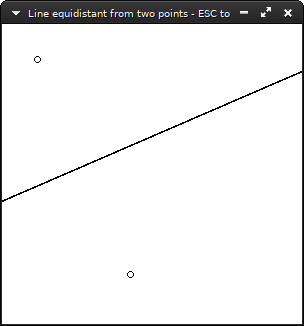
\includegraphics[width=\textwidth,keepaspectratio]{figures/equidistant1.png}
  \end{minipage}
  \hspace{.1em}
  \begin{minipage}{0.49\textwidth}
    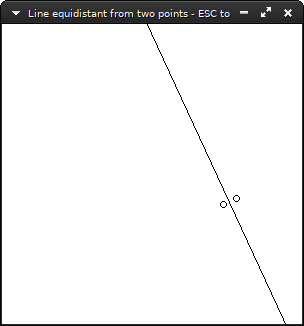
\includegraphics[width=\textwidth,keepaspectratio]{figures/equidistant2.png}
  \end{minipage}
  \Caption{The \texttt{src/bin/equidistant.rs} example has two interactive points and computes their $L_{EQ}$.}
\end{figure}
%
%
%
%
%
\chapter{Reflection of point on line}\index{line!reflection of point}\index{reflection of point}\index{point!reflection on line}\index{mirroring!point to line}
\todo[inline]{Add \emph{Mirror-reflection of point to line}}
\skelpar%
%
%
%
\chapter{Normal to a line through a point}
\todo[inline]{Add \emph{Normal to a line through a point}}
\skelpar%
\chapter{Angle sectioning}
\section{Bisection}\index{angle!bisectioning}
\skelpar%
\section{Trisection}\index{angle!trisectioning}
% http://www.geom.uiuc.edu/docs/forum/angtri/
If the title startled you, be assured it's not a joke. It's totally possible to trisect an angle\ldots{} with a ruler. The adage that angle trisection is impossible refers to using only a compass and unmarked straightedge.

\skelpar%
\clearpage{}
\myaddthumb{Points and Line Segments}{segments}
\part{Points And Line Segments}
\chapter{Drawing a line segment from its two endpoints}

For any line segment with any slope, \pixels{} must be matched with the infinite
amount of points contained in the segment. As shown in the following figure, a segment \emph{touches} some \pixels{}; we could fill them using an algorithm and get a \bitmap{} of the line segment.

\begin{figure}[H]
\centering
\input{figures/fig2.pdf_tex}
\end{figure}

The algorithm presented here was first derived by Bresenham. In the \emph{Image} implementation, it is used in the \texttt{plot\_line\_width} method.
% From graphic gems vol 1 p 99 (pdf page 124)
\begin{minted}{rust}
pub fn plot_line_width(&mut self, (x1, y1): (i64, i64), (x2, y2): (i64, i64)) {
    /* Bresenham's line algorithm */
    let mut d;
    let mut x: i64;
    let mut y: i64;
    let ax: i64;
    let ay: i64;
    let sx: i64;
    let sy: i64;
    let dx: i64;
    let dy: i64;

    dx = x2 - x1;
    ax = (dx * 2).abs();
    sx = if dx > 0 { 1 } else { -1 };

    dy = y2 - y1;
    ay = (dy * 2).abs();
    sy = if dy > 0 { 1 } else { -1 };

    x = x1;
    y = y1;

    let b = dx / dy;
    let a = 1;
    let double_d = (_wd * f64::sqrt((a * a + b * b) as f64)) as i64;
    let delta = double_d / 2;

    if ax > ay {
        d = ay - ax / 2;
        loop {
            self.plot(x, y);
            if x == x2 {
                return;
            }
            if d >= 0 {
                y = y + sy;
                d = d - ax;
            }
            x = x + sx;
            d = d + ay;
        }
    } else {
        d = ax - ay / 2;
        let delta = double_d / 3;
        loop {
            self.plot(x, y);
            if y == y2 {
                return;
            }
            if d >= 0 {
                x = x + sx;
                d = d - ay;
            }
            y = y + sy;
            d = d + ax;
        }
    }
}
\end{minted}
\todo[inline]{Add some explanation behind the algorithm in \emph{Drawing a line segment from its two endpoints}}
\chapter{Drawing line segments with width}
\begin{minted}{rust}
pub fn plot_line_width(&mut self, (x1, y1): (i64, i64), (x2, y2): (i64, i64), _wd: f64) {
    /* Bresenham's line algorithm */
    let mut d;
    let mut x: i64;
    let mut y: i64;
    let ax: i64;
    let ay: i64;
    let sx: i64;
    let sy: i64;
    let dx: i64;
    let dy: i64;

    dx = x2 - x1;
    ax = (dx * 2).abs();
    sx = if dx > 0 { 1 } else { -1 };

    dy = y2 - y1;
    ay = (dy * 2).abs();
    sy = if dy > 0 { 1 } else { -1 };

    x = x1;
    y = y1;

    let b = dx / dy;
    let a = 1;
    let double_d = (_wd * f64::sqrt((a * a + b * b) as f64)) as i64;
    let delta = double_d / 2;

    if ax > ay {
        d = ay - ax / 2;
        loop {
            self.plot(x, y);
            {
                let total = |_x| _x - (y * dx) / dy + (y1 * dx) / dy - x1;
                let mut _x = x;
                loop {
                    let t = total(_x);
                    if t < -1 * delta || t > delta {
                        break;
                    }
                    _x += 1;
                    self.plot(_x, y);
                }
                let mut _x = x;
                loop {
                    let t = total(_x);
                    if t < -1 * delta || t > delta {
                        break;
                    }
                    _x -= 1;
                    self.plot(_x, y);
                }
            }
            if x == x2 {
                return;
            }
            if d >= 0 {
                y = y + sy;
                d = d - ax;
            }
            x = x + sx;
            d = d + ay;
        }
    } else {
        d = ax - ay / 2;
        let delta = double_d / 3;
        loop {
            self.plot(x, y);
            {
                let total = |_x| _x - (y * dx) / dy + (y1 * dx) / dy - x1;
                let mut _x = x;
                loop {
                    let t = total(_x);
                    if t < -1 * delta || t > delta {
                        break;
                    }
                    _x += 1;
                    self.plot(_x, y);
                }
                let mut _x = x;
                loop {
                    let t = total(_x);
                    if t < -1 * delta || t > delta {
                        break;
                    }
                    _x -= 1;
                    self.plot(_x, y);
                }
            }
            if y == y2 {
                return;
            }
            if d >= 0 {
                x = x + sx;
                d = d - ay;
            }
            y = y + sy;
            d = d + ax;
        }
    }
}
\end{minted}
% Graphics gems vol 1. pdf page 139 "RENDERING FAT LINES ON 2D GRID"

\chapter{Intersection of two line segments}
% Graphics gems vol 2. pdf page 37
Let points $\textbf{1}=(x_1,y_1)$, $\textbf{2} = (x_2, y_2)$, $\textbf{3} = (x_3, y_3)$ and $\textbf{4} = (x_4, y_4)$ and $\textbf{1,2}$, $\textbf{3,4}$ two line segments they form. We wish to find their intersection:

First, get the equation of line $L_{12}$ and line $L_{34}$ from chapter \emph{\nameref{ch:equations-lines}}.

Substitute points $\textbf{3}$ and $\textbf{4}$ in equation $L_{12}$ to compute $r_3 = L_{12}(\textbf{3})$ and $r_4=L_{12}(\textbf{4})$ respectively.

If $r_3 \neq{} 0$, $r_4 \neq{} 0$ and $sgn(r_3)==sign(r_4)$ the line segments don't intersect, so stop.

In $L_{34}$ substitute point $\textbf{1}$ to compute $r_1$, and do the same for point $\textbf{2}$.

If $r_1 \neq{} 0$, $r_2 \neq{} 0$ and $sgn(r_1)==sign(r_2)$ the line segments don't intersect, so stop.

At this point, $L_{12}$ and $L_{34}$ either intersect or are equivalent. Find their intersection point. (See \emph{\nameref{ch:intersection-lines}} page \pageref{ch:intersection-lines})
\section{\emph{Fast} intersection of two line segments}
% Graphics gems vol 3. pdf page 231
\skelpar%
\clearpage{}
\myaddthumb{Points, Lines and Circles}{circles}
\part{Points, Lines and Circles}
\skelpar%
\chapter{Equations of a circle}\label{ch:equations-circles}
\todo[inline]{Add \emph{Equations of a circle}}
\index{circle!equations}%
\skelpar%
\chapter{Bounding circle}
\index{circle!bounding}%
% From graphic gems vol 2 pdf page 46
% From Υπολογιστική Γεωμετρία 4.7 page 85 Μικρότατοι περικλείοντες δίσκοι
\attachsource{src/bin/boundingcircle.rs}
\begin{figure}[H]
\centering
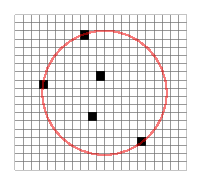
\includegraphics[scale=2,keepaspectratio]{figures/minidisc.pdf}
\end{figure}
A bounding circle is a circle that includes all the points in a given set. Usually we're interested in one of the smallest ones possible.

\begin{figure}[H]
\centering
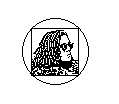
\includegraphics{figures/minidisc.png}
\end{figure}

We can use the following methodology to find the bounding circle: start from two points and the circle they make up, and for each of the rest of the points check if the circle includes them. If not, make a bounding circle that includes every point up to the current one. To do this, we need some primitive operations.

We will need a way to construct a circle out of two points:\index{circle!out of two points}

\begin{figure}[H]
\centering

\includegraphics[scale=0.25,keepaspectratio]{figures/two_points_circle.png}
\end{figure}

\begin{minted}{rust}
  let p1 = points[0];
  let p2 = points[1];
  //The  circle  is  determined  by  two  points,  P  and  Q.  The  center  of the  circle  is
  //at  (P  +  Q)/2.0  and  the  radius  is  |(P  –  Q)/2.0|
  let d_2 = (
  (((p1.0 + p2.0) / 2), (p1.1 + p2.1) / 2),
  (distance_between_two_points(p1, p2) / 2.0),
  );
\end{minted}

And a way to make a circle out of three points:\index{circle!out of three points}

\begin{figure}[H]
\centering
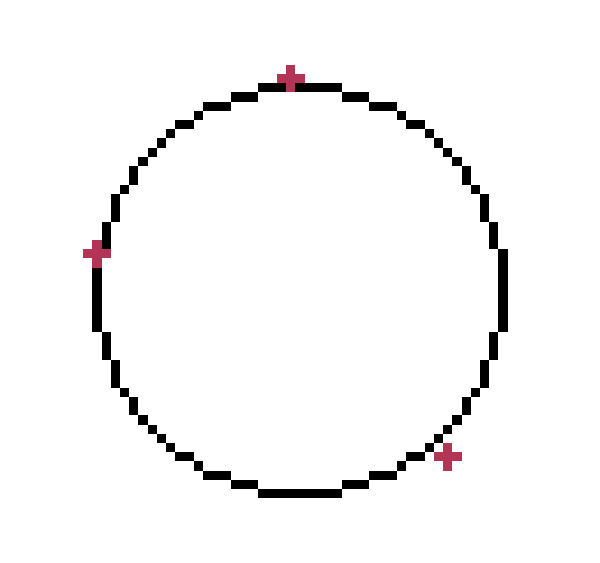
\includegraphics[scale=0.25,keepaspectratio]{figures/triangle_circle.png}
\end{figure}
% graphics gems vol 1. triangles
\begin{minted}{rust}
fn min_circle_w_3_points(q1: Point, q2: Point, q3: Point) -> Circle {
    let (ax, ay) = (q1.0 as f64, q1.1 as f64);
    let (bx, by) = (q2.0 as f64, q2.1 as f64);
    let (cx, cy) = (q3.0 as f64, q3.1 as f64);

    let mut d = 2. * (ax * (by - cy) + bx * (cy - ay) + cx * (ay - by));
    if d == 0.0 {
        d = std::cmp::max(
            std::cmp::max(
                distance_between_two_points(q1, q2) as i64,
                distance_between_two_points(q2, q3) as i64,
            ),
            distance_between_two_points(q1, q3) as i64,
        ) as f64
            / 2.;
    }
    let ux = ((ax * ax + ay * ay) * (by - cy)
        + (bx * bx + by * by) * (cy - ay)
        + (cx * cx + cy * cy) * (ay - by))
        / d;
    let uy = ((ax * ax + ay * ay) * (cx - bx)
        + (bx * bx + by * by) * (ax - cx)
        + (cx * cx + cy * cy) * (bx - ax))
        / d;
    let mut center = (ux as i64, uy as i64);

    if center.0 < 0 {
        center.0 = 0;
    }
    if center.1 < 0 {
        center.1 = 0;
    }
    let d = distance_between_two_points(center, q1);
    (center, d)
}
\end{minted}

The algorithm:

\begin{minted}{rust}
use bitmappers_companion::*;
use minifb::{Key, Window, WindowOptions};
use rand::seq::SliceRandom;
use rand::thread_rng;
use std::f64::consts::{FRAC_PI_2, PI};

include!("../me.xbm.rs");

const WINDOW_WIDTH: usize = 400;
const WINDOW_HEIGHT: usize = 400;

pub fn distance_between_two_points(p_k: Point, p_l: Point) -> f64 {
    let (x_k, y_k) = p_k;
    let (x_l, y_l) = p_l;
    let xlk = x_l - x_k;
    let ylk = y_l - y_k;
    f64::sqrt((xlk * xlk + ylk * ylk) as f64)
}

fn image_to_points(image: &Image) -> Vec<Point> {
    let mut ret = Vec::with_capacity(image.bytes.len());
    for y in 0..(image.height as i64) {
        for x in 0..(image.width as i64) {
            if image.get(x, y) == Some(BLACK) {
                ret.push((x, y));
            }
        }
    }
    ret
}

type Circle = (Point, f64);

fn bc(image: &Image) -> Circle {
    let mut points = image_to_points(image);
    points.shuffle(&mut thread_rng());
    min_circle(&points)
}
fn min_circle(points: &[Point]) -> Circle {
    let mut points = points.to_vec();
    points.shuffle(&mut thread_rng());

    let p1 = points[0];
    let p2 = points[1];
    //The  circle  is  determined  by  two  points,  P  and  Q.  The  center  of the  circle  is
    //at  (P  +  Q)/2.0  and  the  radius  is  |(P  –  Q)/2.0|
    let d_2 = (
        (((p1.0 + p2.0) / 2), (p1.1 + p2.1) / 2),
        (distance_between_two_points(p1, p2) / 2.0),
    );

    let mut d_prev = d_2;

    for i in 2..points.len() {
        let p_i = points[i];
        if distance_between_two_points(p_i, d_prev.0) <= (d_prev.1) {
            // then d_i = d_(i-1)
        } else {
            let new = min_circle_w_point(&points[..i], p_i);
            if distance_between_two_points(p_i, new.0) <= (new.1) {
                d_prev = new;
            }
        }
    }

    d_prev
}

fn min_circle_w_point(points: &[Point], q: Point) -> Circle {
    let mut points = points.to_vec();

    points.shuffle(&mut thread_rng());
    let p1 = points[0];
    //The  circle  is  determined  by  two  points,  P_1  and  Q.  The  center  of the  circle  is
    //at  (P_1  +  Q)/2.0  and  the  radius  is  |(P_1  –  Q)/2.0|
    let d_1 = (
        (((p1.0 + q.0) / 2), (p1.1 + q.1) / 2),
        (distance_between_two_points(p1, q) / 2.0),
    );

    let mut d_prev = d_1;

    for j in 1..points.len() {
        let p_j = points[j];
        if distance_between_two_points(p_j, d_prev.0) <= (d_prev.1) {
            //d_prev = d_prev;
        } else {
            let new = min_circle_w_points(&points[..j], p_j, q);
            if distance_between_two_points(p_j, new.0) <= (new.1) {
                d_prev = new;
            }
        }
    }
    d_prev
}

fn min_circle_w_points(points: &[Point], q1: Point, q2: Point) -> Circle {
    let mut points = points.to_vec();

    let d_0 = (
        (((q1.0 + q2.0) / 2), (q1.1 + q2.1) / 2),
        (distance_between_two_points(q1, q2) / 2.0),
    );

    let mut d_prev = d_0;
    for k in 0..points.len() {
        let p_k = points[k];
        if distance_between_two_points(p_k, d_prev.0) <= (d_prev.1) {
        } else {
            let new = min_circle_w_3_points(q1, q2, p_k);
            if distance_between_two_points(p_k, new.0) <= (new.1) {
                d_prev = new;
            }
        }
    }
    d_prev
}

fn min_circle_w_3_points(q1: Point, q2: Point, q3: Point) -> Circle {
    let (ax, ay) = (q1.0 as f64, q1.1 as f64);
    let (bx, by) = (q2.0 as f64, q2.1 as f64);
    let (cx, cy) = (q3.0 as f64, q3.1 as f64);

    let mut d = 2. * (ax * (by - cy) + bx * (cy - ay) + cx * (ay - by));
    if d == 0.0 {
        d = std::cmp::max(
            std::cmp::max(
                distance_between_two_points(q1, q2) as i64,
                distance_between_two_points(q2, q3) as i64,
            ),
            distance_between_two_points(q1, q3) as i64,
        ) as f64
            / 2.;
    }
    let ux = ((ax * ax + ay * ay) * (by - cy)
        + (bx * bx + by * by) * (cy - ay)
        + (cx * cx + cy * cy) * (ay - by))
        / d;
    let uy = ((ax * ax + ay * ay) * (cx - bx)
        + (bx * bx + by * by) * (ax - cx)
        + (cx * cx + cy * cy) * (bx - ax))
        / d;
    let mut center = (ux as i64, uy as i64);

    if center.0 < 0 {
        center.0 = 0;
    }
    if center.1 < 0 {
        center.1 = 0;
    }
    let d = distance_between_two_points(center, q1);
    (center, d)
}

fn main() {
    let mut buffer: Vec<u32> = vec![WHITE; WINDOW_WIDTH * WINDOW_HEIGHT];
    let mut window = Window::new(
        "Test - ESC to exit",
        WINDOW_WIDTH,
        WINDOW_HEIGHT,
        WindowOptions {
            title: true,
            //borderless: true,
            resize: true,
            //transparency: true,
            ..WindowOptions::default()
        },
    )
    .unwrap();

    // Limit to max ~60 fps update rate
    window.limit_update_rate(Some(std::time::Duration::from_micros(16600)));

    let mut full = Image::new(WINDOW_WIDTH, WINDOW_HEIGHT, 0, 0);
    let mut image = Image::new(ME_WIDTH, ME_HEIGHT, 45, 45);
    image.bytes = bits_to_bytes(ME_BITS, ME_WIDTH);
    let (center, r) = bc(&image);
    image.draw_outline();

    full.plot_circle((center.0 + 45, center.1 + 45), r as i64, 0.);
    while window.is_open() && !window.is_key_down(Key::Escape) && !window.is_key_down(Key::Q) {
        image.draw(&mut buffer, BLACK, None, WINDOW_WIDTH);
        full.draw(&mut buffer, BLACK, None, WINDOW_WIDTH);

        window
            .update_with_buffer(&buffer, WINDOW_WIDTH, WINDOW_HEIGHT)
            .unwrap();

        let millis = std::time::Duration::from_millis(100);

        std::thread::sleep(millis);
    }
}
\end{minted}
\clearpage{}
\myaddthumb{Points, Lines and Shapes}{shapes}
\part{Points, Lines and Shapes}
\chapter{Rectangles and parallelograms}
\skelpar%
\section{From a center point}
\skelpar%
\section{From a corner point}
\chapter{Triangles}\index{triangle}
\skelpar%
\section{Making a triangle from a point and given angles}\index{triangle!from point and angles}
\skelpar%
%\section{Reuleaux triangle}
%https://en.wikipedia.org/wiki/Reuleaux_triangle
\chapter{Union, intersection and difference of polygons}\index{polygon!boolean operations}
\todo[inline]{Add \emph{Union, intersection and difference of polygons}}
% Graphics gems vol 2. pdf page 63
\skelpar%
\chapter{Centroid of polygon}\index{centroid|see {polygon!centroid}}\index{polygon!centroid}\index{centroid!polygon}
\todo[inline]{Add \emph{Centroid of polygon}}
% http://paulbourke.net/geometry/polygonmesh/
% Graphics gems vol 4. pdf page 14
\skelpar%
\chapter{Polygon clipping}\index{polygon!clipping}
% https://github.com/jasonwebb/morphogenesis-resources#polygon-clipping
\skelpar%
\chapter{Triangle filling}\index{triangle!filling}\index{flood filling!triangle filling}
\todo[inline]{Add \emph{Triangle filling} explanation}
\sourceinlib{}%
The book's library methods include a \texttt{fill\_triangle} method:
\begin{minted}{rust}
pub fn fill_triangle(&mut self, q1: Point, q2: Point, q3: Point) {
    let make_equation =
        |p1: Point, p2: Point, p3: Point, a: &mut i64, b: &mut i64, c: &mut i64| {
            *a = p2.1 - p1.1;
            *b = p1.0 - p2.0;
            *c = p1.0 * p2.1 - p1.1 * p2.0;

            if *a * p3.0 + *b * p3.1 + *c < 0 {
                *a = -*a;
                *b = -*b;
                *c = -*c;
            }
        };
    let mut x_min = q1.0;
    let mut y_min = q1.1;
    let mut x_max = q1.0;
    let mut y_max = q1.1;
    let mut a = [0_i64; 3];
    let mut b = [0_i64; 3];
    let mut c = [0_i64; 3];

    // find bounding box
    for q in [q1, q2, q3] {
        x_min = std::cmp::min(x_min, q.0);
        x_max = std::cmp::max(x_max, q.0);

        y_min = std::cmp::min(y_min, q.1);
        y_max = std::cmp::max(y_max, q.1);
    }
    make_equation(q1, q2, q3, &mut a[0], &mut b[0], &mut c[0]);
    make_equation(q1, q3, q2, &mut a[1], &mut b[1], &mut c[1]);
    make_equation(q2, q3, q1, &mut a[2], &mut b[2], &mut c[2]);

    let mut d0 = a[0] * x_min + b[0] * y_min + c[0];
    let mut d1 = a[1] * x_min + b[1] * y_min + c[1];
    let mut d2 = a[2] * x_min + b[2] * y_min + c[2];

    for y in y_min..=y_max {
        let mut f0 = d0;
        let mut f1 = d1;
        let mut f2 = d2;

        d0 += b[0];
        d1 += b[1];
        d2 += b[2];

        for x in x_min..=x_max {
            if f0 >= 0 && f1 >= 0 && f2 >= 0 {
                self.plot(x, y);
            }
            f0 += a[0];
            f1 += a[1];
            f2 += a[2];
        }
    }
}
\end{minted}

\chapter{Flood filling}\index{flood filling}\index{bucket filling|see {flood filling}}\index{area filling|see {flood filling}}
\todo[inline]{Add \emph{Flood filling}}
\skelpar%
% Graphics gems vol 1. pdf page 296 "SEED FILL"
% Graphics gems vol 1. pdf page 299 "FILLING A REGION IN A FRAMEBUFFER"
\clearpage{}
\myaddthumb{Curves other than circles}{curves}
\part{Curves other than circles}
\chapter{Parametric elliptical arcs}\index{curves!elliptical}
\begin{figure}[H]
  \centering
  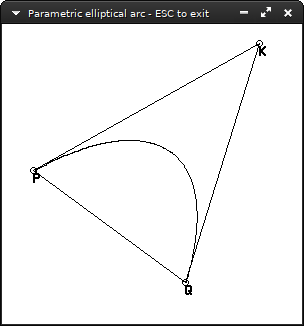
\includegraphics[keepaspectratio]{figures/parellarc.png}
  \Caption{$P$, $Q$ and $K$ are the arc's control points.}
\end{figure}
This algorithm\footnote{\emph{Graphics Gems III} page 164} draws an elliptical arc starting from point $P$ and ending at $Q$. The control point $K$ mirrors the ellipse's center $J$: drawing the quadrilateral $PKQJ$ would appear as a lozenge, or rhombus.

The parameter $t$ defines the step angle in radians and is limited to $0<t\leq{}1$. For each point calculation, the point is $t$ radians away from the previous one, so to increase the amount of points calculated keep $t$ small.
\attachsource{src/bin/parellarc.rs}
\begin{minted}{rust}
fn parellarc(image: &mut Image, p: Point, q: Point, k: Point, t: f64) {
    if t <= 0. || t > 1. {
        return;
    }

    let mut v = ((k.0 - q.0) as f64, (k.1 - q.1) as f64);

    let mut u = ((k.0 - p.0) as f64, (k.1 - p.1) as f64);

    let j = ((p.0 as f64 - v.0 + 0.5), (p.1 as f64 - v.1 + 0.5));

    u = (
        (u.0 * f64::sqrt(1. - t * t * 0.25) - v.0 * t * 0.5),
        (u.1 * f64::sqrt(1. - t * t * 0.25) - v.1 * t * 0.5),
    );

    let n = (std::f64::consts::FRAC_PI_2 / t).floor() as u64;

    let mut prev_pos = p;
    for _ in 0..n {
        let x = (v.0 + j.0).round() as i64;
        let y = (v.1 + j.1).round() as i64;
        let new_point = (x, y);
        image.plot_line_width(prev_pos, new_point, 1.);
        prev_pos = new_point;

        u.0 -= v.0 * t;
        v.0 += u.0 * t;
        u.1 -= v.1 * t;
        v.1 += u.1 * t;
    }
}
\end{minted}

\begin{figure}[H]
  \centering
  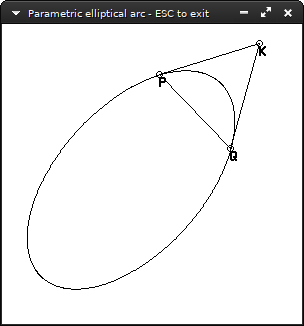
\includegraphics[keepaspectratio]{figures/parellarc2.png}
  \Caption{Changing $n$ to $\frac{2\pi{}}{t}$ draws the entire ellipse.}
\end{figure}
\chapter{Bézier curves}\index{curves!Bézier}
\begin{figure}[H]
\centering
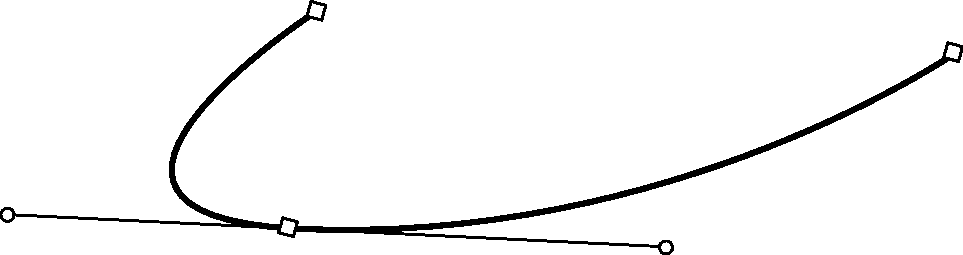
\includegraphics[width=\textwidth,keepaspectratio]{figures/bezier_path.pdf}\par
{\noindent{}Two cubic \emph{Bézier} curves joined together as displayed in graphics software.}
\end{figure}
\skelpar%
\skelpar%
\section{Quadratic Bézier curves}\index{curves!Bézier!quadratic}
\subsection{Drawing the quadratic}
To actually draw a curve, i.e.\ with points $P_1,P_2,P_3$ we will use \emph{de Casteljau's algorithm}\index{de Casteljau's algorithm}. The gist behind the algorithm is that the length of the curve is visited at specific percentages (e.g.\ 0\%, 0.2\%, 0.4\% \ldots{} 99.8\%, 100\%), meaning we will have that many steps, and for each such percentage $t$ we calculate a line starting at the $t$-nth point of $P_{1}P_{2}$ and ending at the $t$-nth point of $P_{2}P_{3}$. The $t$-eth point of that line also belongs to the curve, so we plot it.
\begin{figure}[H]
  \centering
  \begin{minipage}{0.49\textwidth}
    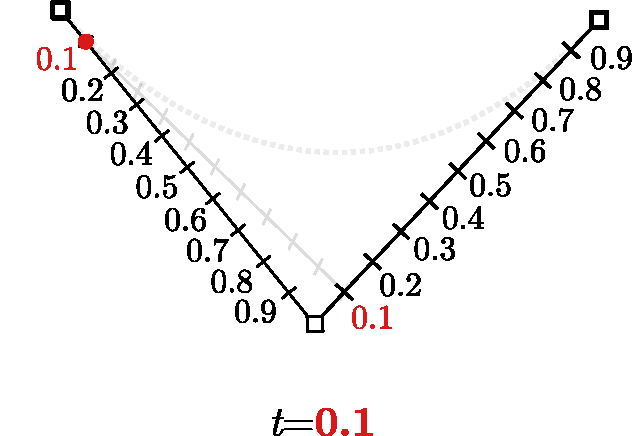
\includegraphics[width=\textwidth,keepaspectratio]{figures/bezier_step_0.1.pdf}
  \end{minipage}
  \hspace{.1em}
  \begin{minipage}{0.49\textwidth}
    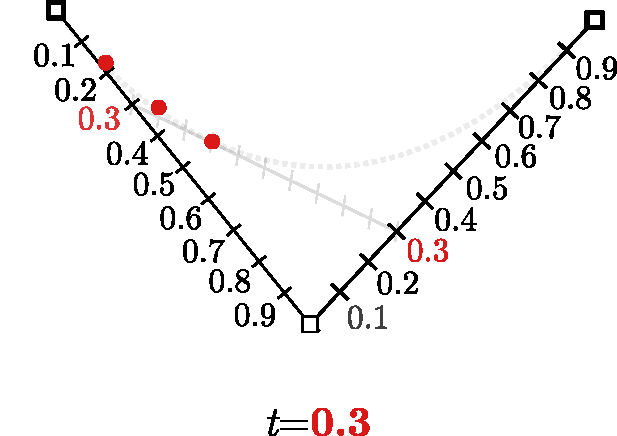
\includegraphics[width=\textwidth,keepaspectratio]{figures/bezier_step_0.3.pdf}
  \end{minipage}
  \par
  \begin{minipage}{0.49\textwidth}
    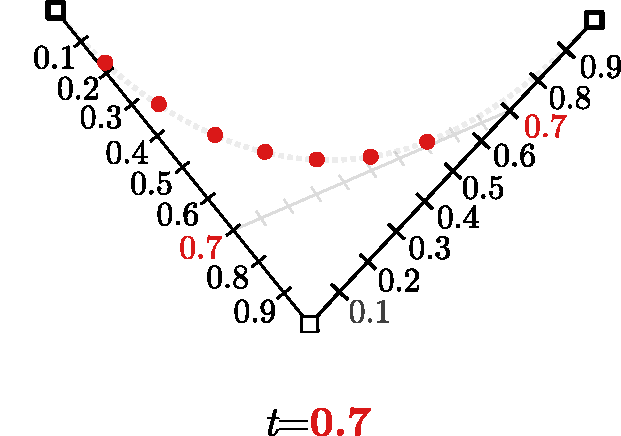
\includegraphics[width=\textwidth,keepaspectratio]{figures/bezier_step_0.7.pdf}
  \end{minipage}
  \hspace{.1em}
  \begin{minipage}{0.49\textwidth}
    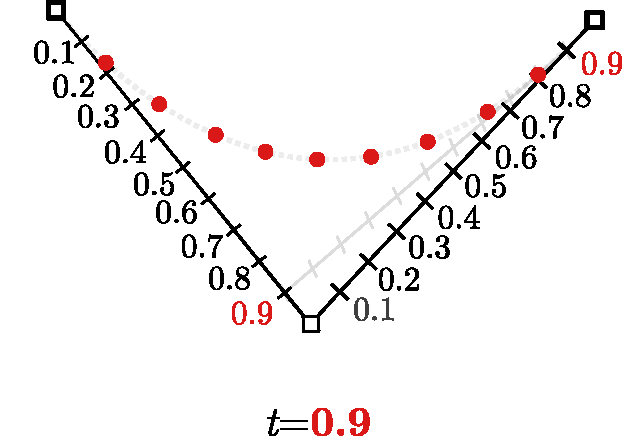
\includegraphics[width=\textwidth,keepaspectratio]{figures/bezier_step_0.9.pdf}
  \end{minipage}\par
  \vspace{1em}
  {\noindent{}Computing curve points for values of $t \in [0, 1]$ with de Casteljau's algorithm}
\end{figure}

Let's draw the curve $P_1= (25, 115), P_2 = (225, 180), P_3 = (250, 25)$
\attachsource{src/bin/bezier.rs}
\begin{minted}{rust}
\end{minted}
The result:
\begin{figure}[H]
\centering
  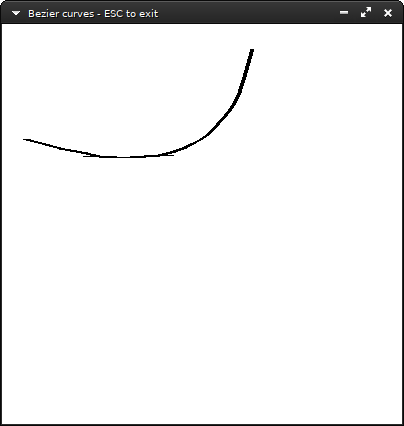
\includegraphics[width=0.5\textwidth,keepaspectratio]{figures/quadratic_drawn.png}
\end{figure}
The \texttt{minifb} library allows to track user input, so we detect user clicks and the mouse's position; thus we can interactively modify a curve with some modifications in the code:
\begin{minted}{rust}
\end{minted}
\skelpar%
\begin{figure}[H]
\centering
  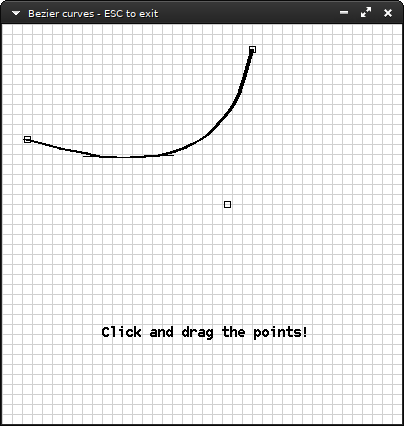
\includegraphics[scale=0.9,keepaspectratio]{figures/quadratic_interactive.png}\par
  \vspace{1em}
  {\noindent{}Interactively modifying a curve with the \texttt{bezier.rs} tool.}
\end{figure}%
We can go one step further and insult type designers\footnote{who use cubic Béziers or other fancier curves (\emph{splines})} and use the tool to make a font glyph.
\attachsource{src/bin/bezierglyph.rs}
\begin{minted}{rust}
\end{minted}
Of course, it requires effort to match the beginning and end of each curve that makes up the glyph. That's why font designing tools have \emph{point snapping} to ensure curve continuation. But for a quick font designer app prototype, it's good enough.
\begin{figure}[H]
\centering
  \begin{minipage}{0.49\textwidth}
    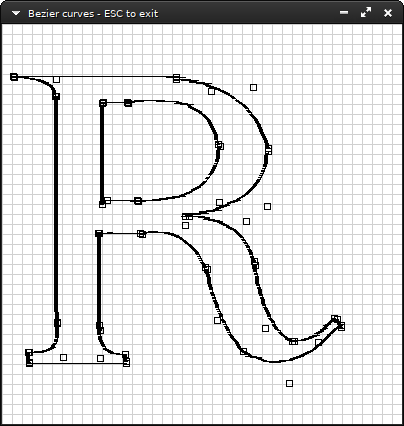
\includegraphics[width=\textwidth,keepaspectratio]{figures/quadratic_glyph.png}
  \end{minipage}
  \hfill
  \begin{minipage}{0.49\textwidth}
    \fbox{
\includegraphics[width=\textwidth,keepaspectratio]{figures/Rglyph.pdf}}
  \end{minipage}\par
  \vspace{1em}
  {\noindent{}\emph{Left}: A font glyph drawn with the interactive \texttt{bezierglyph.rs} tool. \emph{Right}: the same glyph exported to \texttt{SVG}.}
\end{figure}
\clearpage{}
\section{Cubic Bézier curves}\index{curves!Bézier!cubic}
\skelpar%
\section{Weighted Béziers}\index{curves!Bézier!weighted}
\skelpar%
\chapter{Archimedean spiral}
\begin{figure}[H]
  \centering
  
\includegraphics[height=12\baselineskip,keepaspectratio]{figures/archspiral.pdf}
\end{figure}
\section*{The code}
\skelpar
\attachsource{src/bin/archimedeanspiral.rs}
\begin{minted}{rust}
pub fn arch(image: &mut Image, center: Point) {
    let a = 1.0_f64;
    let b = 9.0_f64;

    // max_angle = number of spirals * 2pi.
    let max_angle = 5.0_f64 * 2.0_f64 * std::f64::consts::PI;

    let mut theta = 0.0_f64;
    let (dx, dy) = center;
    let mut prev_point = center;
    while theta < max_angle {
        theta = theta + 0.002_f64;

        let r = a + b * theta;
        let x = (r * theta.cos()) as i64 + dx;
        let y = (r * theta.sin()) as i64 + dy;
        image.plot_line_width(prev_point, (x, y), 1.0);
        prev_point = (x, y);
    }
}
\end{minted}
\begin{figure}[H]
  \centering
  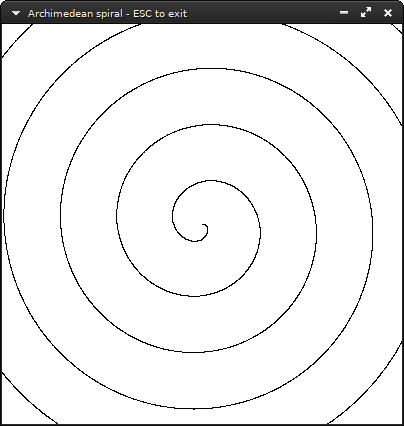
\includegraphics[scale=1,keepaspectratio]{figures/archspiral.png}
\end{figure}
\clearpage{}
\myaddthumb{Vectors, matrices and transformations}{trans\-for\-ma\-tions}
\part{Vectors, matrices and trans\-for\-ma\-tions}
\chapter{Rotation of a \bitmap{}}\index{rotation}

\[
  p' =
  \begin{bmatrix}
    \cos{}θ & -\sin{}θ\\
    \sin{}θ & \cos{}θ
  \end{bmatrix}
  \begin{bmatrix}
    x_{p}\\
    y_{p}
  \end{bmatrix}
\]

\begin{equation*}
  c = \cos{}θ,\\\\
  s = \sin{}θ,\\
  x_{p'} = x_{p}c-y_{p}s,\\
  y_{p'} = x_{p}s+y_{p}c.
\end{equation*}

Let's load an \texttt{xface}. We will use \texttt{bits\_to\_bytes} (See \emph{\nameref{ch:bitstobytes}}, page \pageref{ch:bitstobytes}).
%
\attachsource{src/bin/rotation.rs}%
%
%
\begin{minted}{rust}
include!("dmr.rs");

const WINDOW_WIDTH: usize = 100;
const WINDOW_HEIGHT: usize = 100;

let mut image = Image::new(DMR_WIDTH, DMR_HEIGHT, 25, 25);
image.bytes = bits_to_bytes(DMR_BITS, DMR_WIDTH);
\end{minted}

\begin{figure}[H]
\centering
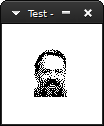
\includegraphics{figures/ch11-1.png}
\end{figure}

This is the \texttt{xface} of \texttt{dmr}. Instead of displaying the \bitmap{}, this time we will rotate it $0.5$ radians. Setup our image first:


\begin{minted}{rust}
let mut image = Image::new(DMR_WIDTH, DMR_HEIGHT, 25, 25);
image.draw_outline();
let dmr = bits_to_bytes(DMR_BITS, DMR_WIDTH);
\end{minted}

And then, loop for each byte in \texttt{dmr}'s face and apply the rotation transformation.

\begin{minted}{rust}
let angle = 0.5;

let c = f64::cos(angle);
let s = f64::sin(angle);

for y in 0..DMR_HEIGHT {
    for x in 0..DMR_WIDTH {
        if dmr[y * DMR_WIDTH + x] == BLACK {
            let x = x as f64;
            let y = y as f64;
            let xr = x * c - y * s;
            let yr = x * s + y * c;
            image.plot(xr as i64, yr as i64);
        }
    }
}
\end{minted}

The result:

\begin{figure}[H]
\centering
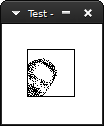
\includegraphics{figures/ch11-2.png}
\end{figure}

We didn't mention in the beginning that the rotation has to be relative to a \emph{point} and the given transformation is relative to the \emph{origin}, in this case the upper left corner $(0,0)$. So \texttt{dmr} was rotated relative to the origin\,:
\begin{figure}[H]
\centering
  \def\svgscale{0.6}
\input{figures/cartesian_grid_dmr_1.pdf_tex}
  \def\svgscale{0.6}
\input{figures/cartesian_grid_dmr_2.pdf_tex}
\end{figure}

{\centering{}
\noindent(the distance to the origin (actually 0 \pixels{}) has been exaggerated for the sake of the example)
}

Usually, we want to rotate something relative to itself. The right point to choose is the \emph{centroid} of the object.\index{centroid!rectangle}

If we have a list of $n$ points, the centroid is calculated as:

$$ x_c = \frac{1}{n}\sum_{i=0}^{n} x_i $$
$$ y_c = \frac{1}{n}\sum_{i=0}^{n} y_i $$

Since in this case we have a rectangle, the centroid has coordinates of half the width and half the height.

By subtracting the centroid from each point before we apply the transformation and then adding it back after we get what we want:

Here's it visually: First subtract the center point.

\begin{figure}[H]
\centering
\def\svgscale{0.6}
\input{figures/cartesian_grid_dmr_3.pdf_tex}
\end{figure}

Then, rotate.

\begin{figure}[H]
\centering
\def\svgscale{0.6}
\input{figures/cartesian_grid_dmr_4.pdf_tex}
\end{figure}

And subtract back to the original position.

\begin{figure}[H]
\centering
\def\svgscale{0.6}
\input{figures/cartesian_grid_dmr_5.pdf_tex}
\end{figure}

In code:

\begin{minted}{rust}
let center_point = ((DMR_WIDTH/2) as i64, (DMR_HEIGHT/2) as i64);
for y in 0..DMR_HEIGHT {
    for x in 0..DMR_WIDTH {
        if dmr[y * DMR_WIDTH + x] == BLACK {
            let x = (x as i64 -center_point.0) as f64;
            let y = (y as i64 -center_point.1) as f64;
            let xr = x * c - y * s;
            let yr = x * s + y * c;
            image.plot(xr as i64+center_point.0,
                       yr as i64 + center_point.1);
        }
    }
}
\end{minted}

The result: 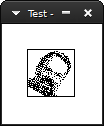
\includegraphics{figures/ch11-3.png}

\section{Fast 2D Rotation}
\todo[inline]{Add \emph{Fast 2D Rotation}}
% Graphics gems vol 1. pdf page 456 
\skelpar%
\chapter{90\textdegree{} Rotation of a \bitmap{} by parallel recursive subdivision}
\todo[inline]{Add \emph{90\textdegree{} Rotation of a \bitmap{} by parallel recursive subdivision}}
% Graphics gems vol 2. pdf page 113 
\skelpar%
\chapter{Magnification/Scaling}\index{magnification}\index{scaling}
\begin{figure}[H]
\centering
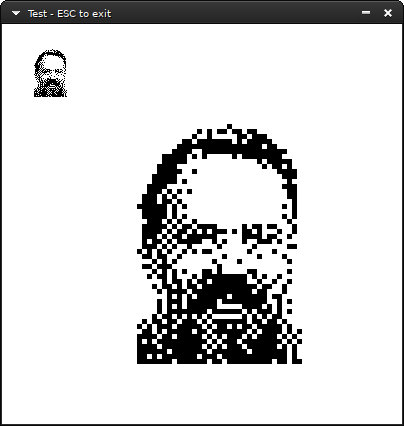
\includegraphics[width=0.5\textwidth,keepaspectratio]{figures/scaled_dmr.png}
\end{figure}
We want to magnify a \bitmap{} without any smoothing. We define an \texttt{Image} scaled to the dimensions we want, and loop for every \pixel{} in the scaled \texttt{Image}. Then, for each \pixel{}, calculate its source in the original \bitmap{}: if the coordinates in the scaled \bitmap{} are $(x, y)$  then the source coordinates $(sx, sy)$ are:

$$ sx = \frac{x * original.width}{scaled.width}$$
$$ sy = \frac{y * original.height}{scaled.height}$$

So, if $(sx, sy)$ are painted, then $(x, y)$ must be painted as well.

\attachsource{src/bin/scale.rs}%
\begin{minted}{rust}
let mut original = Image::new(DMR_WIDTH, DMR_HEIGHT, 25, 25);
original.bytes = bits_to_bytes(DMR_BITS, DMR_WIDTH);
original.draw(&mut buffer, BLACK, None, WINDOW_WIDTH);

let mut scaled = Image::new(DMR_WIDTH * 5, DMR_HEIGHT * 5, 100, 100);
let mut sx: i64; //source
let mut sy: i64; //source
let mut dx: i64; //destination
let mut dy: i64 = 0; //destination

let og_height = original.height as i64;
let og_width = original.width as i64;
let scaled_height = scaled.height as i64;
let scaled_width = scaled.width as i64;

while dy < scaled_height {
    sy = (dy * og_height) / scaled_height;
    dx = 0;
    while dx < scaled_width {
        sx = (dx * og_width) / scaled_width;
        if original.get(sx, sy) == Some(BLACK) {
            scaled.plot(dx, dy);
        }
        dx += 1;
    }
    dy += 1;
}
scaled.draw(&mut buffer, BLACK, None, WINDOW_WIDTH);
\end{minted}
\section{Smoothing enlarged \bitmaps{}}\index{smoothing}
\todo[inline]{Add \emph{Smoothing enlarged \bitmaps{}}}
% https://en.wikipedia.org/wiki/Hqx
% Graphics gems vol 1. pdf page 189 "SMOOTHING ENLARGED MONOCHROME IMAGES"
\skelpar%
\section{Stretching lines of \bitmaps{}}\index{stretching}
\todo[inline]{Add \emph{Stretching lines of \bitmaps{}}}
% Graphics gems vol 3. pdf page 34 "FAST BITMAP STRETCHING"
\skelpar%
\chapter{Mirroring}\index{mirroring}
\todo[inline]{Add screenshots and figure and code in \emph{Mirroring}}
Mirroring to an axis is the transformation of one coordinate to its equidistant value across the axis:

To mirror a \pixel across the $x$ axis, simply multiply its coordinates with the following matrix:

\[
  M_x =
  \begin{bmatrix}
    1 & 0\\
    0 & -1
  \end{bmatrix}
\]

This results in the $y$ coordinate's sign being flipped.

For $y$-mirroring, the transformation follows the same logic:

\[
  M_y =
  \begin{bmatrix}
    -1 & 0\\
    0 & 1
  \end{bmatrix}
\]

% Geometric tools for computer graphics  pdf page 195, "Reflection"
\chapter{Shearing}
\attachsource{src/bin/shearing.rs}%
Simple shearing\index{shearing}\index{skewing|see {shearing}} is the transformation of one dimension by a distance proportional to the other dimension, In $x$-shearing (or horizontal shearing) only the $x$ coordinate is affected, and likewise in $y$-shearing only $y$ as well.

% Geometric tools for computer graphics  pdf page 200, "Shearing"
\begin{figure}[H]
\centering
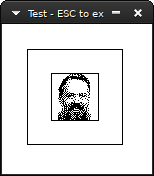
\includegraphics{figures/shearing-0.png}
\end{figure}

With $l$ being equal to the desired tilt away from the $y$ axis, the transformation is described by the following matrix:

\[
  S_x =
  \begin{bmatrix}
    1 & l\\
    0 & 1
  \end{bmatrix}
\]

Which is as simple as this function:

\begin{minted}{rust}
fn shear_x((x_p, y_p): (i64, i64), l: f64) -> (i64, i64) {
    (x_p+(l*(y_p as f64)) as i64, y_p)
}
\end{minted}

\begin{figure}[H]
\centering
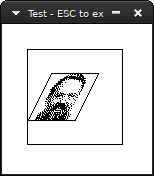
\includegraphics{figures/shearing-1.png}
\end{figure}

For $y$-shearing, we have the following:

\[
  S_y =
  \begin{bmatrix}
    1 & 0\\
    l & 1
  \end{bmatrix}
\]

\begin{minted}{rust}
fn shear_y((x_p, y_p): (i64, i64), l: f64) -> (i64, i64) {
    (x_p, (l*(x_p as f64)) as i64 + y_p)
}
\end{minted}

\begin{figure}[H]
\centering
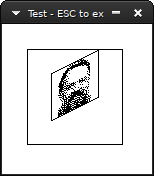
\includegraphics{figures/shearing-2.png}
\end{figure}

A full example:
\begin{minted}{rust}
include!("../dmr.xbm.rs");

const WINDOW_WIDTH: usize = 200;
const WINDOW_HEIGHT: usize = 200;

fn shear_x((x_p, y_p): (i64, i64), l: f64) -> (i64, i64) {
    (x_p+(l*(y_p as f64)) as i64, y_p)
}
fn shear_y((x_p, y_p): (i64, i64), l: f64) -> (i64, i64) {
    (x_p, (l*(x_p as f64)) as i64 + y_p)
}

let mut image = Image::new(DMR_WIDTH, DMR_HEIGHT, 25, 25);
image.bytes = bits_to_bytes(DMR_BITS, DMR_WIDTH);
image.draw_outline();

let l = -0.5;
let mut sheared = Image::new(DMR_WIDTH*2, DMR_HEIGHT*2, 25, 25);
for x in 0..DMR_WIDTH {
    for y in 0..DMR_HEIGHT  {
        if image.bytes[y * DMR_WIDTH + x] == BLACK {
          let p = shear_x((x as i64 ,y as i64 ), l);
          sheared.plot(p.0+(DMR_WIDTH/2) as i64, p.1+(DMR_HEIGHT/2) as i64); 
        }
    }
}
sheared.draw_outline();
\end{minted}
\section{The relationship between shearing factor and angle}
\begin{figure}[H]
\centering
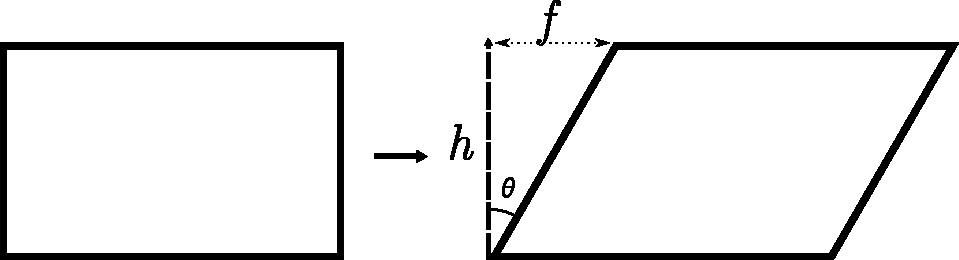
\includegraphics[width=\textwidth,keepaspectratio]{figures/xshear.pdf}
\end{figure}
Shearing is a delta movement in one dimension, thus the point before moving and the point after form an angle with the $x$ axis. To move a point $(x, 0)$ by 30\textdegree{} forward we will have the new point $(x+f, 0)$ where $f$ is the shear factor. These two points and $(x, h)$ where $h$ is the height of the \bitmap{} form a triangle, thus the following are true:

$$\cot\theta{} = \frac{h}{f}$$

Therefore to find your factor for any angle $\theta{}$ replace its cotangent in the following formula:

$$f = \frac{h}{\cot\theta{}}$$

For example to shear by $-$30\textdegree{} (meaning the \bitmap{} will move to the right, since rotations are always clockwise) we need $\cot(-30deg) = -\sqrt{3}$ and $f=-\frac{h}{\sqrt{3}}$.

\chapter{Projections}
\todo[inline]{Add \emph{Projections}}
% Geometric tools for computer graphics  pdf page 205, "Projections"
\skelpar%
\clearpage{}
\myaddthumb{Addendum}{ad\-den\-dum}
\part{Addendum}
\chapter{Faster drawing a line segment from its two endpoints using symmetry}
\todo[inline]{Add \emph{Faster drawing a line segment from its two endpoints using symmetry}}
% From graphic gems vol 1 p 103 (pdf page 128)
\skelpar%
\chapter{Joining the ends of two wide line segments together}
\todo[inline]{Add \emph{Joining the ends of two wide line segments together}}
% Graphics gems vol 1. pdf page 132 "AN ALGORITHM FOR FILLING IN 2D WIDE LINE BEVEL JOINTS"
\begin{figure}[H]
  \centering
    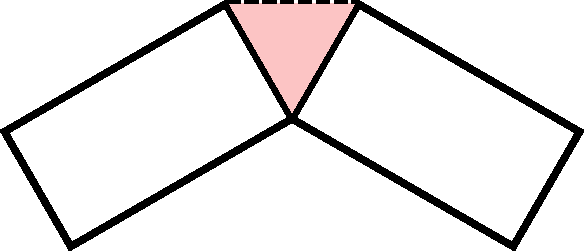
\includegraphics[width=0.48\textwidth,keepaspectratio]{figures/join_beams.pdf}
\end{figure}
\skelpar%
\chapter{Composing monochrome \bitmaps{} with separate alpha channel data}\index{alpha channel}
\todo[inline]{Add \emph{Composing monochrome \bitmaps{} with separate alpha channel data}}
% Graphics gems vol 3. pdf page 64 "COMPOSING BW BITMAPS
\skelpar%
\chapter{Orthogonal connection of two points}
\todo[inline]{Add \emph{Orthogonal connection of two points}}
% Graphics gems vol 3. pdf page 205 "SIMPLE CONNECTION ALGORITHM FOR 2D DRAWING"
\skelpar%
\chapter{Join segments with round corners}\label{ch:roundcorners}
% Graphics gems vol 3. pdf page 225 "JOINING TWO LINES WITH A CIRCULAR ARC FILLET"
\begin{wrapfigure}{r}{0.5\textwidth}
    \vspace{-60pt}
  \begin{center}
    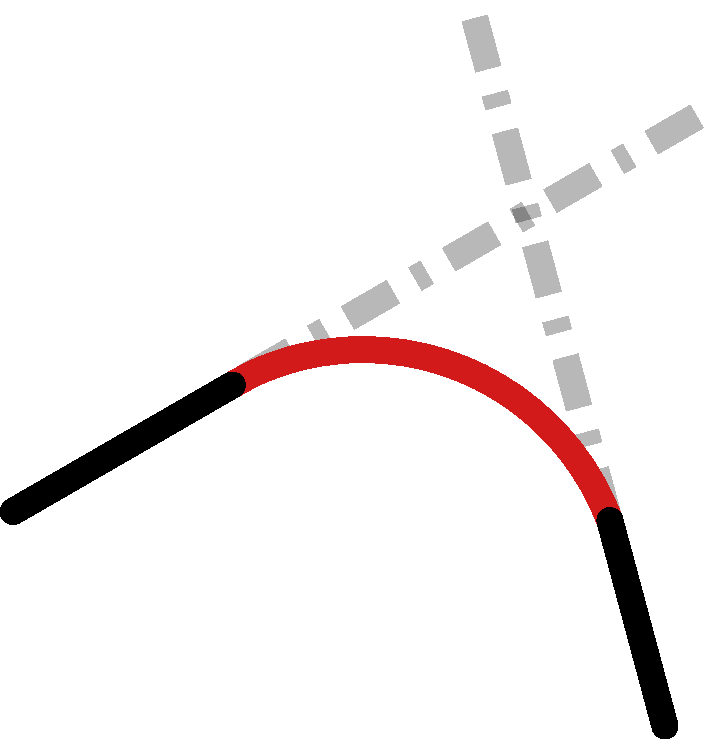
\includegraphics[width=0.48\textwidth,keepaspectratio]{figures/fillet_main.pdf}
  \end{center}
\end{wrapfigure}
Round corners are everywhere around us. It is useful to know at least one method of construction. This specific method constructs a circle that has a common point with each given line segment, and calculates the arc that when added to the line segments they are smoothly joined. The excess length, since those common points will be before the end of the line segments, must be erased. Therefore, it's best to begin with just the points of the two segments before starting to draw anything.

Since the segments intercept, the round corner will end up beneath the intersection. We wish to find a circle
that has a common point with each segment and the arc made up from those points and the circle is the round corner we are after.

\begin{figure}[H]%
  \centering{}%
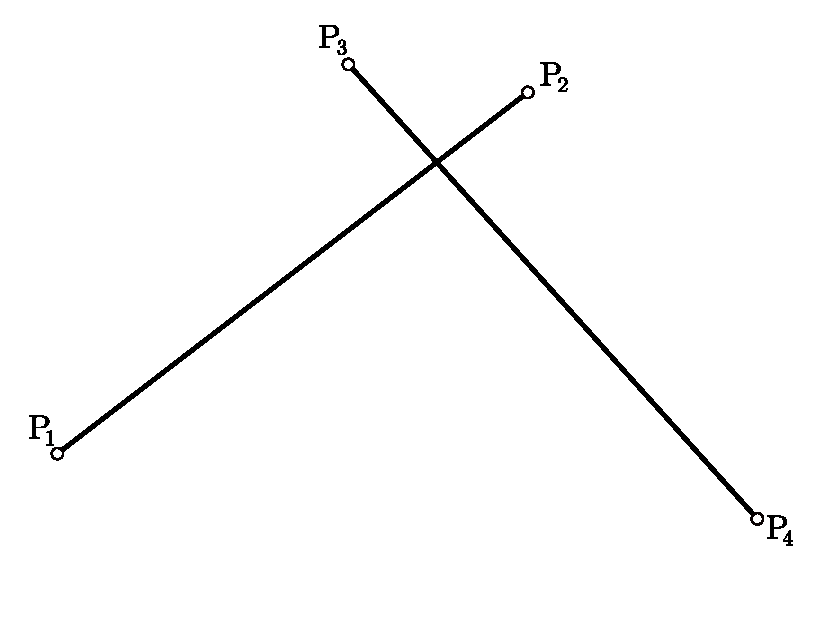
\includegraphics[width=\textwidth,keepaspectratio]{figures/fillet_1.pdf}%
\end{figure}%
%
\noindent{}We are given 4 points, $P_{1}, P_{2}$ and $P_{3}, P_{4}$ that make up segments $S_1$ and $S_2$.
Begin by finding the midpoints $m_1$ and $m_2$ of segments $S_1$ and $S_2$.\index{midpoint} These will be:

$$m_1 = \frac{P_1 + P_2}{2}$$
$$m_2 = \frac{P_3 + P_4}{2}$$

\noindent{}Then, find the signed distances (i.e.\ don't use the absolute value of distance) $d_1$ of $m_1$ from $S_2$ and $d_2$ of $m_2$ from $S_1$.

\noindent{}Construct parallel lines $l_1$ to $S_1$ that is $d_1$ pixels away. Repeat with $l_2$ for $S_2$ and $d_2$.

\noindent{}Their intersection is the circle's center, $P_c$.%

\noindent{}The intersection of $l_1$, $l_2$ with the two segments are the points where we should clip or extend the segments: $q_1$ and $q_2$.

\begin{figure}[H]
  \centering{}
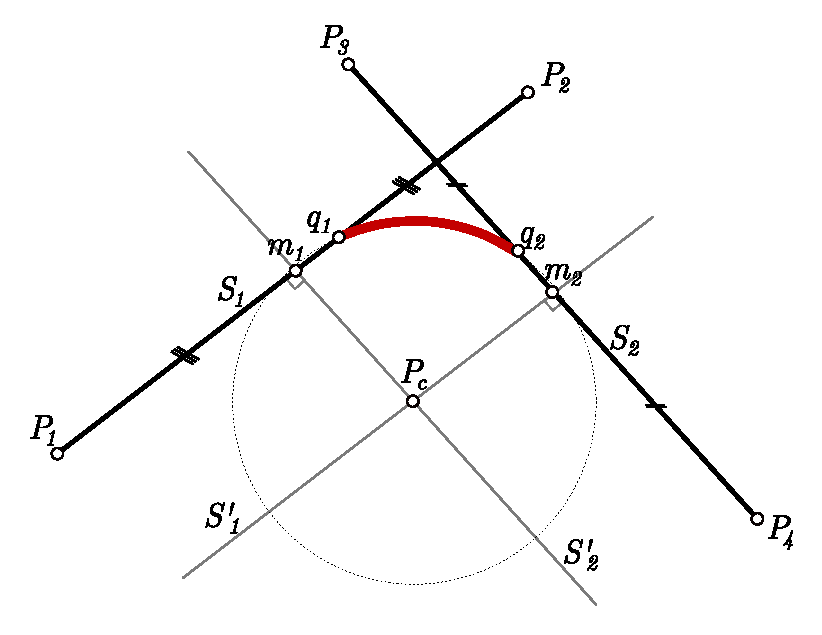
\includegraphics[width=0.8\textwidth,keepaspectratio]{figures/fillet_2.pdf}
\end{figure}

\noindent{}The starting angle is found by calculating the angle of $q_1P_c$ with the $x$-axis with the \texttt{atan2} math library procedure.

\begin{figure}[H]
  \centering{}
  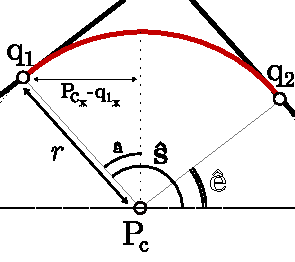
\includegraphics[width=0.8\textwidth,keepaspectratio]{figures/fillet_3.pdf}
\end{figure}

\noindent{}The \emph{subtended} angle\footnote{the \emph{subtended} angle of an arc $\archat{AC}$ to a point $P$ is the angle between $PA$ and $PC$: \raisebox{-1em}{
\includegraphics[scale=4]{figures/subtended_angle.pdf}}} of the arc from the center $P_c$ is found by calculating the dot product of $q_1P_c$ and $q_2P_c$:

\attachsource{src/bin/roundcorner.rs}\noindent{}The code:
\begin{minted}{rust}
\end{minted}
%\noindent{}Calculate perpendicular lines\footnote{See \emph{\nameref{ch:perpendicular}}, page \pageref{ch:perpendicular}} $S'_1$ and $S'_2$ passing through the midpoints of $S_1$ and $S_2$.
%
%\begin{figure}[H]
%  \centering{}
%  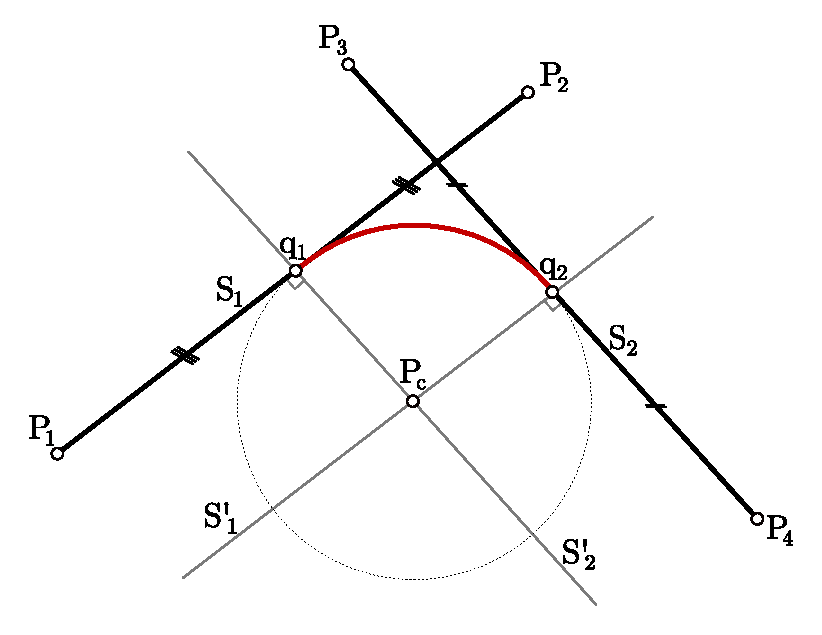
\includegraphics[width=\textwidth,keepaspectratio]{figures/fillet.pdf}
%\end{figure}
%
%
%\noindent{}At their intersection lies the center $P_c$ of the circle, and the radius is the distance of $P_c$ from either of the segments. Now, we have to find the angle the circle's arc starts from. It will be equal to:
%
%$$\hat{s} = 90^{\circ} + \hat{a}$$
%$$\hat{a} = \arcsin\left(\frac{dist_x(P_c, q_1)}{r}\right)$$
%
%\noindent{}Similarly, the ending angle \textbf{\textcolor{white}{\cm{}\LARGE\contour{black}{ê}}} will be equal to:
%
%$$\hat{e} = \arccos\left(\frac{dist_x(P_c, q_2)}{r}\right)$$
%
%\noindent{}It's evident our solution applies to the example and is not general; to cover all cases, we have to find in which quadrants of the circle the wanted arc will reside in and that depends on how the two segments are layed out.

\begin{figure}[H]
  \centering{}
  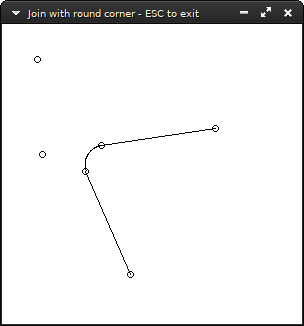
\includegraphics[width=0.5\textwidth,keepaspectratio]{figures/roundcorner1.png}
  \Caption{The \texttt{src/bin/roundcorner.rs} example has two interactive lines and computes the joining fillet.}
\end{figure}
%
%
%
\chapter{Squircle}
\begin{figure}[H]
\centering

\includegraphics[height=5\baselineskip,keepaspectratio]{figures/squircle.pdf}
\end{figure}
\attachsource{src/bin/squircle.rs}
A \emph{squircle} is a compromise between a square and a circle. It is purported to be more pleasing to the eye because the rounding corner is smoother than that of a circle arc (like the result of \emph{\nameref{ch:roundcorners}}, page \pageref{ch:roundcorners}).

A way to describe a squircle is as a superellipse, meaning a generalization of the ellipse equation $\frac{x^2}{a^2} + \frac{y^2}{b^2} = 1$ by making the exponent parametric:
$${\left| x-a \right|}^{n} + {\left| y-b \right|}^{n} = 1$$
The squircle as a superellipse is usually defined for $n=4$.
\section*{The code}
\begin{minted}{rust}
pub fn plot_squircle(
    image: &mut Image,
    (xm, ym): (i64, i64),
    width: i64,
    height: i64,
    n: i32,
    _wd: f64,
) {
    let r = width / 2;
    let w = width / 2;
    let h = height / 2;

    let mut prev_pos = (xm - w, xm - h);

    for i in 0..(2 * r + 1) {
        let x: i64 = (i - r) + w;
        let y: i64 = ((r as f64).powi(n) - (i as f64 - r as f64).abs().powi(n)).powf(1. / n as f64)
            as i64
            + h;
        if i != 0 {
            image.plot_line_width(prev_pos, (xm - x as i64, ym - y), _wd);
        }
        prev_pos = (xm - x as i64, ym - y);
    }
    for i in (2 * r)..(4 * r + 1) {
        let x: i64 = (3 * r - i) + w;
        let y = -1
            * (((r as f64).powi(n) - ((3 * r - i) as f64).abs().powi(n)).powf(1. / n as f64))
                as i64
            + h;
        image.plot_line_width(prev_pos, (xm - x as i64, ym - y), _wd);
        prev_pos = (xm - x as i64, ym - y);
    }
}
\end{minted}
%\thispagestyle{empty}
\section*{Different values of $n$}
Increasing $n$ in \texttt{src/bin/squircle.rs} makes the hyperellipse corners approach the square's.
\begin{figure}[H]
  \centering
  \begin{minipage}{0.49\textwidth}
    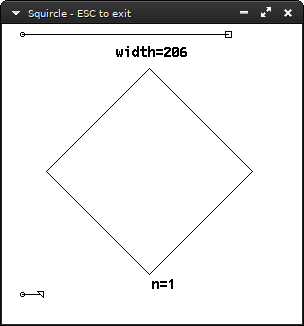
\includegraphics[width=\textwidth,keepaspectratio]{figures/squircle_1.png}
  \end{minipage}
  \hspace{.1em}
  \begin{minipage}{0.49\textwidth}
    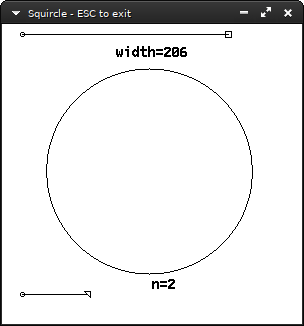
\includegraphics[width=\textwidth,keepaspectratio]{figures/squircle_2.png}
  \end{minipage}
\end{figure}
\begin{figure}[H]
  \centering
  \begin{minipage}{0.49\textwidth}
    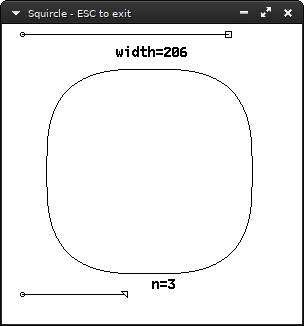
\includegraphics[width=\textwidth,keepaspectratio]{figures/squircle_3.png}
  \end{minipage}
  \hspace{.1em}
  \begin{minipage}{0.49\textwidth}
    \includegraphics[width=\textwidth,keepaspectratio]{figures/squircle_4.png}
  \end{minipage}
\end{figure}
\begin{figure}[H]
  \centering
  \includegraphics[width=0.49\textwidth,keepaspectratio]{figures/squircle_8.png}\par
\end{figure}
%
%
%
%
%
%
%
%
\chapter{Faster line clipping}
\todo[inline]{Add \emph{Faster line clipping}}
% Graphics gems vol 5. pdf page 323 "FASTER PIXEL PERFECT LINE CLIPPING"
\skelpar%
\chapter{Tilings}
\todo[inline]{Add \emph{Tilings}}
\section{Hexagon Tiling}
\chapter{Space-filling Curves}\index{curves!space-filling}
\todo[inline]{Add \emph{Space-filling Curves}}
% https://en.wikipedia.org/wiki/Space-filling_tree maybe?
% Spiral tilings? https://isohedral.ca/escher-like-spiral-tilings/
% Graphics gems vol 2. pdf page 58
\skelpar%
\clearpage{}
\section{Hilbert curve}\index{Hilbert curve}\index{curves!Hilbert curve}
\todo[inline]{Add \emph{Hilbert curve} explanation}
\begin{figure}[H]
\centering
  \includegraphics[height=15\baselineskip,keepaspectratio]{figures/HilbertCurve.pdf}\par
  {\scriptsize{}The first six iterations of the Hilbert curve \myurl{https://commons.wikimedia.org/wiki/File:Hilbert\_curve.svg}{by \texttt{Braindrain0000}}}
\end{figure}
\attachsource{src/bin/hilbert.rs}
Here's a simple algorithm for drawing a Hilbert curve.\footnote{Griffiths, J. G. (1985). \emph{Table-driven algorithms for generating space-filling curves}. Computer-Aided Design, 17(1), 37–41. \texttt{doi:10.1016/0010-4485(85)90009-0}}
\begin{minted}{rust}
const HILBERT: &[&[usize]] = &[
    &[22, 10, 16, 38],
    &[10, 22, 24, 48],
    &[44, 36, 30, 18],
    &[36, 44, 42, 28],
];

fn curve(img: &mut Image, k: usize, order: i64, mut x: i64, mut y: i64) -> (i64, i64) {
    const STEP_SIZE: i64 = 5;
    let mut row: usize;
    let mut direction: usize;
    if order > 0 {
        for j in 0..4 {
            let step = HILBERT[k][j];
            row = (step / 10) - 1;
            let (xn, yn) = curve(img, row, order - 1, x, y);
            x = xn;
            y = yn;
            direction = step % 10;
            let prev = (x, y);
            match direction {
                8 => {
                    // null op
                }
                2 => {
                    //N
                    y -= STEP_SIZE;
                }
                1 => {
                    // NE
                    y -= STEP_SIZE;
                    x += STEP_SIZE;
                }
                0 => {
                    //E
                    x += STEP_SIZE;
                }
                7 => {
                    //SE
                    x += STEP_SIZE;
                    y += STEP_SIZE;
                }
                6 => {
                    //S
                    y += STEP_SIZE;
                }
                5 => {
                    //SW
                    y += STEP_SIZE;
                    x -= STEP_SIZE;
                }
                4 => {
                    //W
                    x -= STEP_SIZE;
                }
                3 => {
                    //NW
                    y -= STEP_SIZE;
                    x -= STEP_SIZE;
                }
                other => unreachable!("{}", other),
            }
            img.plot_line_width(prev, (x, y), 0.);
        }
    }
    (x, y)
}
\end{minted}
\begin{minted}{rust}
let mut image = Image::new(WINDOW_WIDTH, WINDOW_WIDTH, 0, 0);
curve(&mut image, 0, 7, 0, WINDOW_WIDTH as i64);
\end{minted}
\begin{figure}[H]
\centering
  \includegraphics[keepaspectratio,scale=1]{figures/hilbert.png}
\end{figure}
\section{Sierpiński curve}
\begin{figure}[H]
  \centering
  \includegraphics[keepaspectratio,scale=1]{figures/sierpinshi.png}
\end{figure}

Switching the table from the Hilbert implementation to this:

\begin{minted}{rust}
const SIERP: &[&[usize]] = &[
    &[17, 25, 33, 41],
    &[17, 20, 41, 18],
    &[25, 36, 17, 28],
    &[33, 44, 25, 38],
    &[41, 12, 33, 48],
];
\end{minted}
And switching two lines from the function to
\begin{minted}{diff}
 - let step = HILBERT[k][j];
 - row = (step / 10) - 1;
 + let step = SIERP[k][j];
 + row = (step / 10);
\end{minted}
You can draw a Sierpinshi curve of order $n$ by calling \texttt{curve(\&mut image, 0,n+1, 0, 0)}.
\section{Peano curve}\index{Peano curve}\index{curves!Peano curve}
\todo[inline]{Add \emph{Peano curve}}
\section{Z-order curve}
\begin{figure}[H]
  \centering
  \includegraphics[width=\textwidth,keepaspectratio]{figures/Zordercurve.pdf}
\end{figure}
Drawing the Z-order curve is really simple: first, have a counter variable that starts from zero and is incremented by one at each step. Then, you extract the $(x, y)$ coordinates the new step represents from its binary representation. The bits for the $x$ coordinate are located at the odd bits, and for $y$ at the even bits. I.e.\ the values are interleaved as bits in the value of the step:
\begin{figure}[H]
  \centering
  \includegraphics[width=\textwidth,keepaspectratio]{figures/zcurvebits.pdf}
\end{figure}

Knowing this, implementing the drawing process will consist of computing the next step, drawing a line segment from the current step and the next, set the current step as the next and continue;

\begin{minted}{rust}
fn zcurve(img: &mut Image, x_offset: i64, y_offset: i64) {
    const STEP_SIZE: i64 = 8;
    let mut sx: i64 = 0;
    let mut sy: i64 = 0;
    let mut b: u64 = 0;

    let mut prev_pos = (sx + x_offset, sy + y_offset);
    loop {
        let next = b + 1;
        sx = 0;
        if (next & 1) as i64 > 0 {
            sx += STEP_SIZE;
        }
        if next & 0b100 > 0 {
            sx += 2 * STEP_SIZE;
        }
        if next & 0b10_000 > 0 {
            sx += 4 * STEP_SIZE;
        }
        if next & 0b1_000_000 > 0 {
            sx += 8 * STEP_SIZE;
        }
        if next & 0b100_000_000 > 0 {
            sx += 16 * STEP_SIZE;
        }
        if next & 0b10_000_000_000 > 0 {
            sx += 32 * STEP_SIZE;
        }
        if next & 0b1_000_000_000_000 > 0 {
            sx += 64 * STEP_SIZE;
        }
        if next & 0b100_000_000_000_000 > 0 {
            sx += 128 * STEP_SIZE;
        }
        if next & 0b10_000_000_000_000_000 > 0 {
            sx += 256 * STEP_SIZE;
        }
        if next & 0b1_000_000_000_000_000_000 > 0 {
            sx += 512 * STEP_SIZE;
        }
        sy = 0;
        if (next & 0b10) as i64 > 0 {
            sy += STEP_SIZE;
        }
        if next & 0b1_000 > 0 {
            sy += 2 * STEP_SIZE;
        }
        if next & 0b100_000 > 0 {
            sy += 4 * STEP_SIZE;
        }
        if next & 0b10_000_000 > 0 {
            sy += 8 * STEP_SIZE;
        }
        if next & 0b1_000_000_000 > 0 {
            sy += 16 * STEP_SIZE;
        }
        if next & 0b100_000_000_000 > 0 {
            sy += 32 * STEP_SIZE;
        }
        if next & 0b10_000_000_000_000 > 0 {
            sy += 64 * STEP_SIZE;
        }
        if next & 0b1_000_000_000_000_000 > 0 {
            sy += 128 * STEP_SIZE;
        }
        if next & 0b100_000_000_000_000_000 > 0 {
            sy += 256 * STEP_SIZE;
        }
        if next & 0b10_000_000_000_000_000_000 > 0 {
            sy += 512 * STEP_SIZE;
        }
        img.plot_line_width(prev_pos, (sx + x_offset, sy + y_offset), 1.0);

        if next == 0b111_111_111_111_111_111_111_111 {
            break;
        }
        if sx as usize > img.width && sy as usize > img.height {
            break;
        }

        prev_pos = (sx + x_offset, sy + y_offset);
        b = next;
    }
}
\end{minted}
\begin{figure}[H]
  \centering
  \includegraphics[width=0.3\textwidth,keepaspectratio]{figures/zcurve.png}
\end{figure}
\clearpage{}
\section{Flowsnake curve}\index{Flowsnake curve}\index{Gosper curve|see {Flowsnake curve}}\index{curves!Flowsnake curve}
% https://en.wikipedia.org/wiki/Gosper_curve
\begin{figure}[H]
  \centering
  \begin{minipage}{\textwidth}
  \begin{minipage}{0.30\textwidth}
    \hfill
    \includegraphics[width=\textwidth,keepaspectratio]{figures/gosper1.pdf}
    \hfill
  \end{minipage}
  \hspace{0.028\textwidth}
  \begin{minipage}{0.30\textwidth}
    \hfill
    \includegraphics[width=\textwidth,keepaspectratio]{figures/gosper2.pdf}
    \hfill
  \end{minipage}
  \hspace{0.028\textwidth}
  \begin{minipage}{0.30\textwidth}
    \hfill
    \includegraphics[width=\textwidth,keepaspectratio]{figures/gosper3.pdf}
    \hfill
  \end{minipage}
  \end{minipage}\par
  \vspace{1em}
  {\noindent{}The first three orders of the Gosper curve.}
\end{figure}
As a fractal curve, the \emph{flowsnake curve} or \emph{Gosper curve} is defined by a set of recursive rules for drawing it. There are four kind of rules and two of them define rulesets (i.e.\ they are non-terminal steps).

% http://paulbourke.net/fractals/lsys/index.html L-System User Notes
\begin{align*}
A\mapsto{}&\,A{-}B{-}{-}B{+}A{+}{+}AA{+}B{-}\\
B\mapsto{}&{+}A{-}BB{-}{-}B{-}A{+}{+}A{+}B
\end{align*}
\skelpar%
\clearpage{}
\thispagestyle{empty}
\hfill
\begin{figure}[H]
  \centering
  \includegraphics[width=\textwidth,keepaspectratio]{figures/gosper4.pdf}\par
  \vspace{1em}
  {\noindent{}The fourth order Gosper curve consists of a minimum of 2057 distinct line segments (but our algorithm draws 36015)}
\end{figure}
\hfill
\clearpage{}
\chapter{Dithering}\index{dithering}
\clearpage{}
%\skelpar%
% https://beyondloom.com/blog/dither.html
% https://tannerhelland.com/2012/12/28/dithering-eleven-algorithms-source-code.html
% http://www.thetenthplanet.de/archives/5367
\section{Floyd-Steinberg}\index{dithering!Floyd-Steinberg}\index{Floyd-Steinberg dithering}
\begin{figure}[H]
  \centering
  \includegraphics[width=\textwidth,keepaspectratio]{figures/floyd_dithering_lake_closeup.jpg}\par
  {\scriptsize{}detail of a standard test image, \myurl{https://sipi.usc.edu/database/database.php?volume=misc&image=12}{\emph{Sailboat on lake}}, with Floyd-Steinberg dithering}
\end{figure}
\skelpar
\attachsource{src/bin/floyddither.rs}
\begin{minted}{rust}
fn floyd(image: &mut Image) {
    let w = image.width;
    let m = [(0, 7), (w - 2, 3), (w - 1, 5), (w, 1)];
    let mut e = vec![0.0; w + 1];
    let bytes = image
        .bytes
        .iter()
        .map(|&byte| {
            let (r, g, b) = from_u32_rgb(byte);
            let g: f64 = (0.299 * (r as f64)) + (0.587_f64 * (g as f64)) + (0.114 * (b as f64));
            let pix = g / 255.0 + {
                e.push(0.);
                e.remove(0)
            };
            let col = if pix > 0.5 { 1. } else { 0. };
            let err = (pix - col) / 16.;
            for (x, y) in m.iter() {
                e[*x] += err * (*y as f64);
            }
            if col.floor() as u32 == 1 {
                WHITE
            } else {
                BLACK
            }
        })
        .collect::<Vec<u32>>();
    image.bytes = bytes;
}
\end{minted}
\begin{figure}[H]
  \centering
  \begin{minipage}{0.48\textwidth}
    \includegraphics[width=\textwidth,keepaspectratio]{figures/4.2.06.jpg}
  \end{minipage}
  \hspace{.4em}
  \begin{minipage}{0.48\textwidth}
    \includegraphics[width=\textwidth,keepaspectratio]{figures/floyd_dithering_lake.png}
  \end{minipage}
\end{figure}
\section{Atkinson dithering}\index{dithering!Atkinson}\index{Atkinson dithering}
\begin{figure}[H]
  \centering
  \includegraphics[width=\textwidth,keepaspectratio]{figures/atkinson_dithering_lena_closeup.jpg}\par
  {\scriptsize{}detail of a standard test image, \myurl{https://en.wikipedia.org/wiki/Lenna}{\emph{Lenna}}, with Atkinson dithering}
\end{figure}
\skelpar

\attachsource{src/bin/atkinsondither.rs}
The following code implements Atkinson dithering:\footnote{Algorithm taken from \myurl{https://beyondloom.com/blog/dither.html}{https://beyondloom.com/blog/dither.html}}
\begin{minted}{rust}
fn atkinson(image: &mut Image) {
    let w= image.width;
    let mut e = vec![0.0;2*w];
    let m = [0, 1, w-2, w-1, w, 2*w-1];
    for byte in image.bytes.iter_mut() {
        let (r,g,b) = from_u32_rgb(*byte);
        let g:f64 = ((0.299*(r as f64)) ) + ((0.587_f64*(g as f64)) ) + ((0.114*(b as f64)) );
        let pix = g/255.0 + { e.push(0.); e.remove(0)};
        let col = if pix > 0.5 { 1. } else { 0. };
        let err = (pix-col)/8.;
        for m in m.iter() {
            e[*m] += err;
        }
        *byte = if (col.floor() as u32 == 1) {
            WHITE
        } else {
            BLACK
        };
    }
}
\end{minted}
\begin{figure}[H]
  \centering
  \begin{minipage}{0.48\textwidth}
  \includegraphics[width=\textwidth,keepaspectratio]{figures/lenna.jpg}
  \end{minipage}
  \hspace{.4em}
  \begin{minipage}{0.48\textwidth}
  \includegraphics[width=\textwidth,keepaspectratio]{figures/atkinson_dithering_lena.png}
  \end{minipage}
\end{figure}
\chapter{Marching squares}\index{marching squares}\index{contour|see {marching squares}}
% https://github.com/jasonwebb/morphogenesis-resources#marching-squares
\skelpar%
\TheEnd{}
\clearpage{}
\stopthumb
\backmatter
\bookmarksetup{startatroot}
\cleardoublepage
\printindex
\cleardoublepage
\bookmarksetup{startatroot}
\colophontitle{About this text}
\pdfbookmark{About this text}{colophon}
\thispagestyle{empty}
\colophontitlesize{25pt}
\begin{colophon}
\noindent{}The text has been typeset in {\cm{}\XeLaTeX{}} using the \texttt{book} class and:
\begin{itemize}
  \item \textbf{Redaction} for the main text.
  \item \textbf{\fira{}Fira Sans} for referring to the programming language \Rust{}\,.
  \item \textbf{\pixelfont{}Redaction20} for referring to the words \bitmap{} and \pixels{} as a concept.
\end{itemize}
\end{colophon}
\clearpage{}
\listoftodos{}
\end{document}
